\chapter{Desarrollo del sistema}
    \label{chapter:desarrollo}

    \chapquote{¿Quién dijo miedo habiendo hospitales?}{Sabiduría popular de la ETSISI}

    En este capítulo se detallan los aspectos más destacados relativos a la implementación del sistema propuesto.

    \section{Infraestructura del proyecto}

        En primer lugar, se han creado dos repositorios en \textit{GitHub} para albergar la implementación del sistema, uno para cada componente principal. El código de la aplicación se encuentra en \href{https://github.com/Emotional-Wellbeing/App}{Emotional-Wellbeing/App}, mientras que el del servidor se encuentra en \href{https://github.com/Emotional-Wellbeing/Api}{Emotional-Wellbeing/Api}, siendo  \textit{VicDominguez} el usuario del autor.

        Debido a que el código de este proyecto ha sido utilizado como base para la realización de otro \gls{tfm} \cite{marco_pinar_desarrollo_2024}, en el repositorio de la aplicación móvil fueron creadas dos ramas (dominguez y dominguez\_debug) que contienen única y exclusivamente el código desarrollado en el marco de este proyecto. En el caso del componente servidor, si bien no fue creada una rama en exclusiva para este \gls{tfm}, todo el código fue creado en este proyecto a excepción del relativo al \textit{user\_databg}, el cual pertenece al alcance del \gls{tfm} \cite{marco_pinar_desarrollo_2024}.
        
        \textit{GitHub} permite acceder fácilmente al historial de \textit{commits} donde se puede visualizar la autoría, la fecha y el contenido de cada actualización, como refleja en la Figura \ref{figure:desarrollo:historial_commits}. Además, gracias al uso del sistema \textit{GitHub Actions}, se implementaron \textit{pipelines} de integración y distribución continuas (CI/CD) en ambos repositorios, los cuales se pueden encontrar en \href{https://github.com/Emotional-Wellbeing/App/tree/dominguez_debug/.github/workflows}{App - ./github/workflows} y \href{https://github.com/Emotional-Wellbeing/API/tree/main/.github/workflows}{Api - ./github/workflows} respectivamente. Si bien no es frecuente su uso en metodologías tradicionales ha sido implementado en este \gls{tfm} ya que permite la realización automática de ciertas acciones.

        \begin{figure}[h]
            \centering
            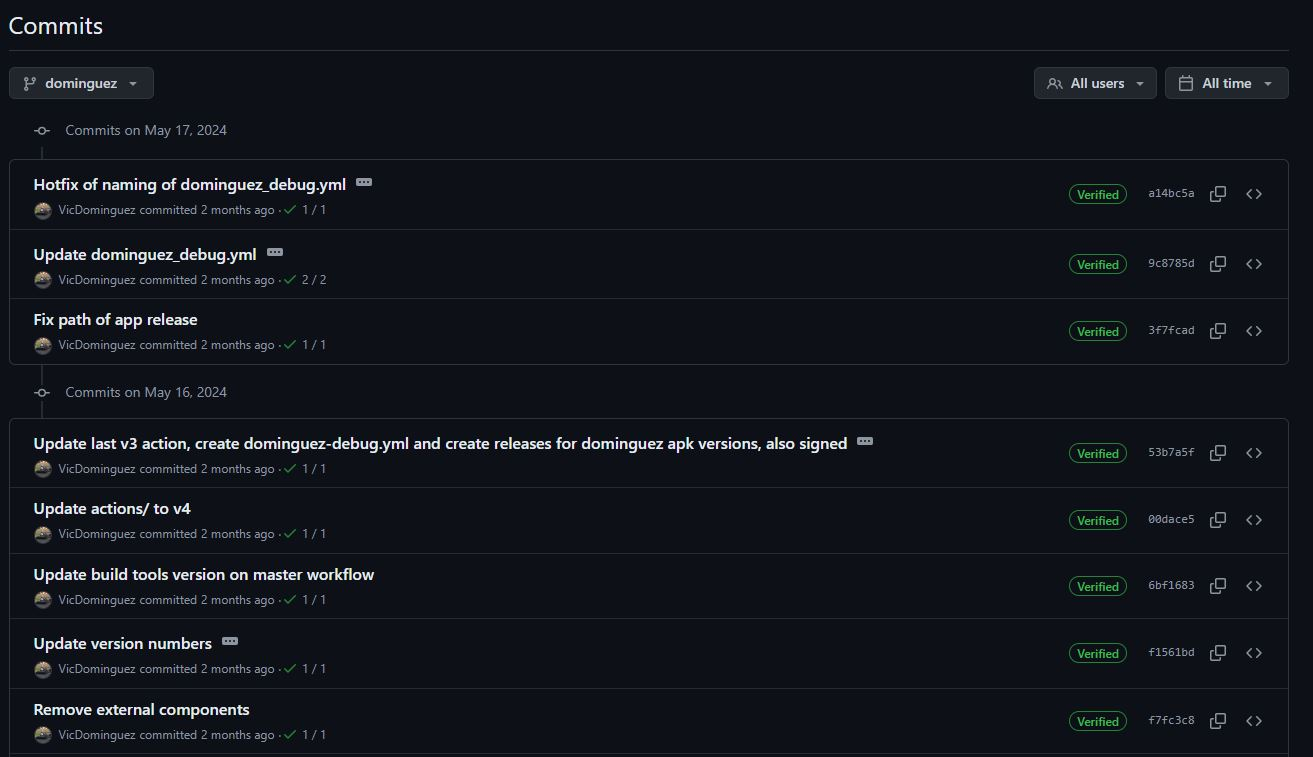
\includegraphics[width=1\textwidth]{figures/desarrollo/commits repo.JPG}
            \caption{Historial de \textit{commits} en el repositorio de la aplicación}
            \label{figure:desarrollo:historial_commits}
        \end{figure}

        En el caso del repositorio de la aplicación, el \textit{pipeline} desempeña las siguientes tareas en cada \textit{commit}:
        \begin{itemize}
            \item Compilación del código en un archivo \gls{apk}.
            \item Ejecución de pruebas automáticas.
            \item Publicación del archivo \gls{apk} compilado durante 90 días.
            \item Publicación del informe de pruebas durante 90 días.
        \end{itemize}

        Además, en el caso de los \textit{commits} etiquetados con el prefijo 'v', se crea una \textit{release} que mantiene la publicación de los archivos por tiempo indefinido. La última \textit{release} se puede visualizar en la Figura \ref{figure:desarrollo:ultima_release} y es accesible mediante el siguiente \href{https://github.com/Emotional-Wellbeing/App/releases/tag/v1.4.0d}{enlace}.

        \begin{figure}[h]
            \centering
            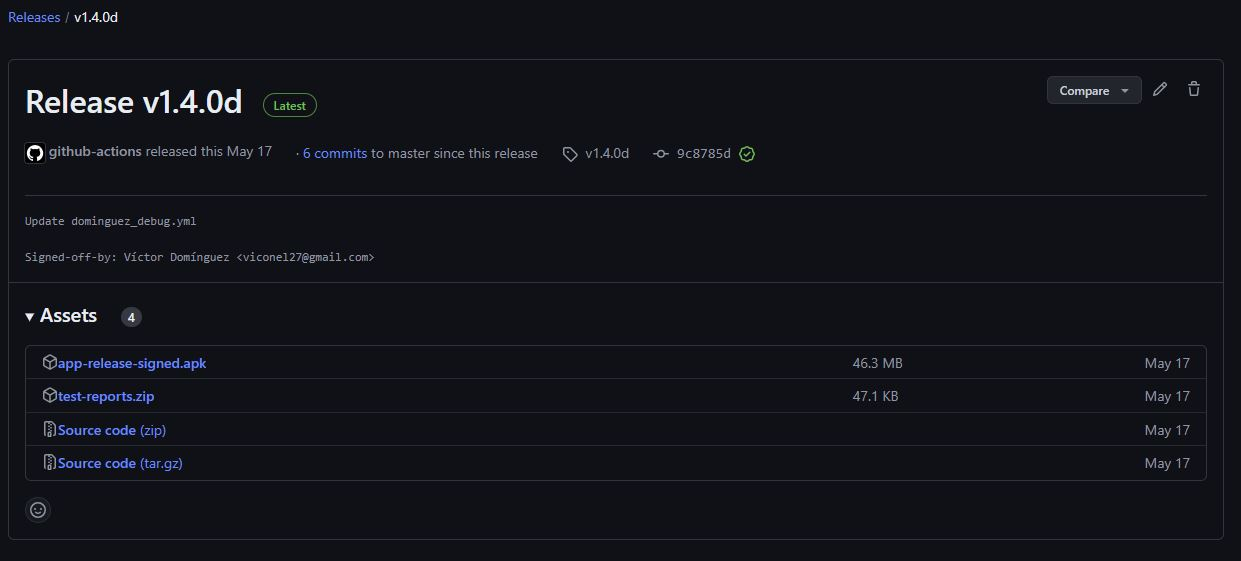
\includegraphics[width=1\textwidth]{figures/desarrollo/ultima release.JPG}
            \caption{Publicación de la \textit{release} v1.4.0d}
            \label{figure:desarrollo:ultima_release}
        \end{figure}
        
        Respecto al repositorio del servidor, el \textit{pipeline} realiza las siguientes tareas en cada \textit{commit}:
        \begin{itemize}
            \item Ejecución de pruebas estáticas mediante \textit{flake8}.
            \item Ejecución de pruebas automáticas y generación del reporte de \textit{coverage}.
            \item Publicación del informe de pruebas durante 90 días.
        \end{itemize}
        
    
    \section{Aplicación móvil}
    
        En esta sección se detallarán únicamente las cuestiones no cubiertas en la fase de diseño o \textit{detalles de implementación}.
        
        \subsection{Grafos de navegación}
            Debido a la gran cantidad de pantallas\footnote{Se utilizarán indistintamente los términos ventana o pantalla para aliviar la notación.} con las que cuenta la aplicación, en este apartado se detalla el grafo de navegación entre las mismas. Para mejorar la legibilidad el grafo se ha dividido en cuatro partes: \textit{primer uso}, \textit{principal}, \textit{cuestionarios diarios} y \textit{cuestionarios puntuales}.

            El grafo \textit{primer uso}, representado en la Figura \ref{figure:disenio:grafo_primer_uso}, resulta muy similar a lo planteado en el diagrama de secuencia correspondiente, el cual fue representado en la Figura \ref{figure:diagrama_secuencia:primer_uso}. La única novedad en ese sentido es la incorporación de la pantalla \textit{splash}, que hace las veces de pantalla de introducción o carga.
            
            \begin{figure}[h]
                \centering
                \begin{tikzpicture}[
                        > = stealth, % estilo de la cabeza de la flecha
                        shorten > = 1pt, % para que la flecha no toque el nodo
                        node distance = 3cm, % distancia entre nodos
                    ]
            
                    \tikzstyle{every state}=[
                        draw = black,
                        thick,
                        fill = white,
                    ]
            
                    \node[rectangle,draw] (click) {\textit{El usuario entra en la app}};
                    \node[state] [below of=click] (splash) {Splash};
                    \node[state] [below of=splash] (bienvenida) {Bienvenida};
                    \node[state] [below of=bienvenida] (permisos) {Permisos};
                    \node[state] [below of=permisos] (inicio) {\textit{Inicio}};
                    
                    \path[->] (click) edge node {} (splash);
                    \path[->] (splash) edge node {} (bienvenida);
                    \path[->] (bienvenida) edge node {} (permisos);
                    \path[->] (permisos) edge node {} (inicio);
            
                \end{tikzpicture}
                \caption{Grafo de navegación \textit{primer uso}}
                \label{figure:disenio:grafo_primer_uso}
            \end{figure}

            En cuanto a la representación del grafo de navegación, la cabeza de las flechas determina el sentido de la navegación, mientras los nodos en cursiva hacen referencia a pantallas descritas en otros grafos. Asimismo, los elementos rectangulares describen el evento activador del grafo en cuestión.
            
            En cuanto al grafo \textit{principal} descrito en la Figura \ref{figure:disenio:grafo_principal}, este detalla las conexiones entre las pantallas que se pueden acceder en cualquier momento. En el caso entre \textit{Inicio} y \textit{Cuestionarios incompletos} solo se puede navegar en el caso que existan cuestionarios incompletos, navegación condicional indicada con la línea discontinua.
            
            \begin{figure}[h]
                \centering
                \begin{tikzpicture}[
                        font=\small, % fuente de letra pequeña
                        > = stealth, % estilo de la cabeza de la flecha
                        shorten > = 1pt, % para que la flecha no toque el nodo
                        node distance = 3.3cm, % distancia entre nodos
                    ]
            
                    \tikzstyle{every state}=[
                        draw = black,
                        thick,
                        fill = white,
                    ]
            
                    \node[rectangle,draw] (click) {\textit{El usuario entra en la app}};
                    \node[state] [below of=click] (splash) {Splash};
                    \node[state] [below of=splash] (inicio) {Inicio};
            
                    \node[state] [below left of=inicio] (historial) {Historial};
                    \node[state] [below right of=inicio] (comunidad) {Comunidad};
                    \node[state, align=center] [right of=inicio] (incompletos) {Cuestionarios\\incompletos};
                    \node[state] [below right of=historial] (ajustes) {Ajustes};
                    \node[state] [left of=inicio] (consejo) {Consejo};
                    \node[state] [left of=historial] (medida) {Medida};
                
                    \node[state, align=center] [above right of=incompletos] (diaria) {\textit{Ronda}\\\textit{diaria}};
                    \node[state, align=center] [below right of=incompletos] (puntual) {\textit{Ronda}\\\textit{puntual}};
                    
                    \node[state] [below of=ajustes] (bienvenida) {Bienvenida};
                    \node[state] [left of=bienvenida] (mis_datos) {Mis datos};
                    \node[state] [left of=mis_datos] (privacidad) {Privacidad};
                    \node[state] [right of=bienvenida] (acerca) {Acerca de};
                    \node[state] [right of=acerca] (créditos) {Créditos};
            
                    \path[->] (click) edge node {} (splash);
                    \path[->] (splash) edge node {} (inicio);
                    
                    \path[<->] (inicio) edge node {} (historial);
                    \path[<->] (inicio) edge node {} (comunidad);
                    \path[<->] (inicio) edge node {} (ajustes);
                    \path[<->] (inicio) edge node {} (medida);
                    \path[<->] (inicio) edge node {} (consejo);
                    \path[<->, dashed] (inicio) edge node {} (incompletos);
            
                    \path[<->] (historial) edge node {} (medida);
                    \path[<->] (historial) edge node {} (comunidad);
                    \path[<->] (historial) edge node {} (ajustes);
                    
                    \path[<->] (ajustes) edge node {} (comunidad);
                    \path[<->] (ajustes) edge node {} (bienvenida);
                    \path[<->] (ajustes) edge node {} (mis_datos);
                    \path[<->] (ajustes) edge node {} (privacidad);
                    \path[<->] (ajustes) edge node {} (acerca);
                    \path[<->] (ajustes) edge node {} (créditos);
                    
                    \path[->] (incompletos) edge node {} (diaria);
                    \path[->] (incompletos) edge node {} (puntual);
            
                \end{tikzpicture}
                \caption{Grafo de navegación \textit{principal}}
                \label{figure:disenio:grafo_principal}
            \end{figure}

            Respecto al grafo de navegación \textit{cuestionarios diarios}, visible en la Figura \ref{figure:disenio:grafo_diario}, este hace referencia a las rondas de cuestionarios diarias descritas en la fase de diseño. La navegación discontinua denota que sólo se podrá navegar a los cuestionarios que el usuario necesite rellenar, pudiendo ser cualquiera de ellos según las circunstancias concretas.

            Por otra parte, \textit{ronda diaria} se trata de un nodo especial, ya que no se corresponde con una \textit{pantalla} visible para el usuario sino de una pantalla \textit{invisible} que contiene la lógica de la ronda de cuestionarios. 
            
            \begin{figure}[h]
                \centering
                \begin{tikzpicture}[
                        font=\small, % fuente de letra pequeña
                        > = stealth, % estilo de la cabeza de la flecha
                        shorten > = 1pt, % para que la flecha no toque el nodo
                        node distance = 3cm, % distancia entre nodos
                    ]
            
                    \tikzstyle{every state}=[
                        draw = black,
                        thick,
                        fill = white,
                    ]
            
                    \node[state, align=center] (diaria) {Ronda\\diaria}; 
            
                    \node[rectangle,draw, align=center] [above left of=diaria] (notificacion) {\textit{El usuario pulsa}\\\textit{en la notificación}};
                    \node[rectangle,draw, align=center] [above right of=diaria] (incompletos) {\textit{El usuario pulsa en un} \\ \textit{cuestionario incompleto}};
                    
                    \node[state] [right of=diaria] (inicio) {\textit{Inicio}}; 
                    
                    \node[state, align=center] [below of=diaria] (suicidio_diario) {Suicidio\\diario};
                    \node[state, align=center] [left of=suicidio_diario] (depresion_diario) {Depresión\\diario};
                    \node[state, align=center] [left of=depresion_diario] (estres_diario) {Estrés\\diario};
                    \node[state, align=center] [right of=suicidio_diario] (soledad_diario) {Soledad\\diario};
                    \node[state, align=center] [right of=soledad_diario] (contraste_diario) {Contraste\\ diario};
            
                    \node[state] [below of=suicidio_diario] (consejo) {Consejo};
            
                    \path[->] (notificacion) edge node {} (diaria);
                    \path[->] (incompletos) edge node {} (diaria);
                    \path[->] (diaria) edge node {} (inicio);
                    \path[<->,dashed] (diaria) edge node {} (estres_diario);
                    \path[<->,dashed] (diaria) edge node {} (depresion_diario);
                    \path[<->,dashed] (diaria) edge node {} (soledad_diario);
                    \path[<->,dashed] (diaria) edge node {} (suicidio_diario);
                    \path[<->,dashed] (diaria) edge node {} (contraste_diario);
            
                    
                    \path[<->] (consejo) edge node {} (estres_diario);
                    \path[<->] (consejo) edge node {} (depresion_diario);
                    \path[<->] (consejo) edge node {} (soledad_diario);
                    \path[<->] (consejo) edge node {} (suicidio_diario);
            
                \end{tikzpicture}
                \caption{Grafo de navegación \textit{cuestionarios diarios}}
                \label{figure:disenio:grafo_diario}
            \end{figure}

            Por último, sobre el grafo de navegación \textit{cuestionarios puntuales} representado en la Figura \ref{figure:disenio:grafo_puntuales}, aplican los mismos razonamientos que se describieron en el grafo de \textit{cuestionarios diarios}.
            
            \begin{figure}[h]
                \centering
                \begin{tikzpicture}[
                        font=\small, % fuente de letra pequeña
                        > = stealth, % estilo de la cabeza de la flecha
                        shorten > = 1pt, % para que la flecha no toque el nodo
                        node distance = 3.5cm, % distancia entre nodos
                    ]
            
                    \tikzstyle{every state}=[
                        draw = black,
                        thick,
                        fill = white,
                    ]
                    
                    \node[state, align=center] (puntual) {Ronda\\puntual}; 
                    
                    \node[rectangle,draw, align=center] [above left of=diaria] (notificacion) {\textit{El usuario pulsa}\\\textit{en la notificación}};
                    \node[rectangle,draw, align=center] [above right of=diaria] (incompletos) {\textit{El usuario pulsa en un} \\ \textit{cuestionario incompleto}};
                    
                    \node[state] [right of=diaria] (inicio) {\textit{Inicio}}; 
                    
                    \node[state, align=center] [below of=puntual] (depresion_puntual) {Depresión\\puntual};
                    \node[state, align=center] [left of=depresion_puntual] (estres_puntual) {Estrés\\puntual};
                    \node[state, align=center] [right of=depresion_puntual] (soledad_puntual) {Soledad\\puntual};
            
                    \node[state] [below of=depresion_puntual] (consejo) {Consejo};
            
                    \path[->] (puntual) edge node {} (inicio);
                    \path[->] (notificacion) edge node {} (puntual);
                    \path[->] (incompletos) edge node {} (puntual);
                    
                    \path[<->,dashed] (puntual) edge node {} (estres_puntual);
                    \path[<->,dashed] (puntual) edge node {} (depresion_puntual);
                    \path[<->,dashed] (puntual) edge node {} (soledad_puntual);
            
                    \path[<->] (consejo) edge node {} (estres_puntual);
                    \path[<->] (consejo) edge node {} (depresion_puntual);
                    \path[<->] (consejo) edge node {} (soledad_puntual);
            
                \end{tikzpicture}
                \caption{Grafo de navegación \textit{cuestionarios puntuales}}
                \label{figure:disenio:grafo_puntuales}
            \end{figure}

            \clearpage  % Asegura que todas las figuras y tablas pendientes se impriman antes de continuar.

        \subsection{Descripción de alto nivel de las pantallas implementadas}
            \label{section:implementacion:pantallas}

            \subsubsection*{\textit{Splash}}
                Esta pantalla, como se puede ver en la Figura \ref{figure:implementacion:pantalla:splash}, cuenta únicamente con el logo de la aplicación y un fondo con el color principal. Se muestra únicamente durante un segundo en cada arranque de la aplicación. 
                \begin{figure}[h]
                	\centering
                	
\includegraphics[width=0.4\textwidth]{figures/pantallas/Splash.png}
                	\caption{Pantalla \textit{splash}}
                	\label{figure:implementacion:pantalla:splash}
                \end{figure}

                \clearpage  % Asegura que todas las figuras y tablas pendientes se impriman antes de continuar.
            \subsubsection*{Bienvenida}

                Esta ventana cuenta con un carrousel de mensajes de bienvenida, presentándose cada uno con un titular y con una animación. El primer mensaje del carrousel se puede visualizar en la Figura \ref{figure:implementacion:pantalla:bienvenida}.
                
                \begin{figure}[h]
                	\centering
                	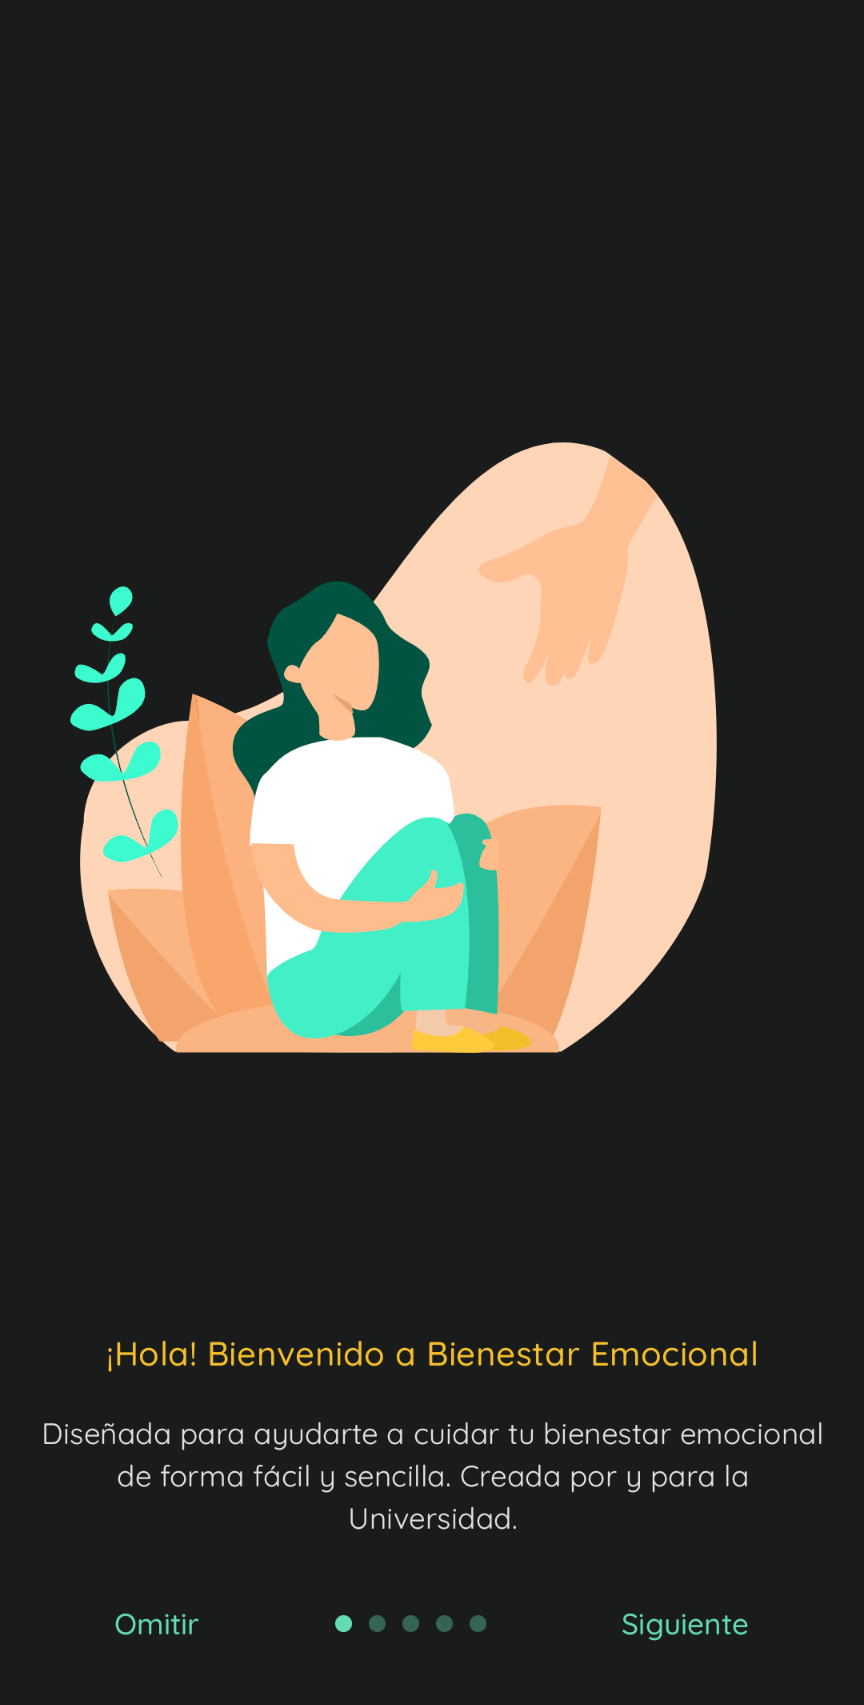
\includegraphics[width=0.4\textwidth]{figures/pantallas/Onboarding 1.png}
                	\caption{Pantalla bienvenida}
                	\label{figure:implementacion:pantalla:bienvenida}
                \end{figure}
                
                \clearpage  % Asegura que todas las figuras y tablas pendientes se impriman antes de continuar.
            \subsubsection*{Permisos}

                En esta pantalla, representada en la Figura \ref{figure:implementacion:pantalla:permisos} se explica al usuario por qué la aplicación necesita ciertos permisos y los enlaces a las ventanas o diálogos de Android para otorgar los permisos en cuestión. Además la ventana cuenta con un botón de continuar para cuando el usuario ha terminado de otorgar permisos.

                Asimismo se trata de una pantalla \textit{básica}, la cual cuenta con un encabezado y con una barra de navegación para acceder a las ventanas principales\footnote{Las ventanas principales son inicio, historial, comunidad y ajustes.}.
                
                \begin{figure}[h]
                	\centering
                	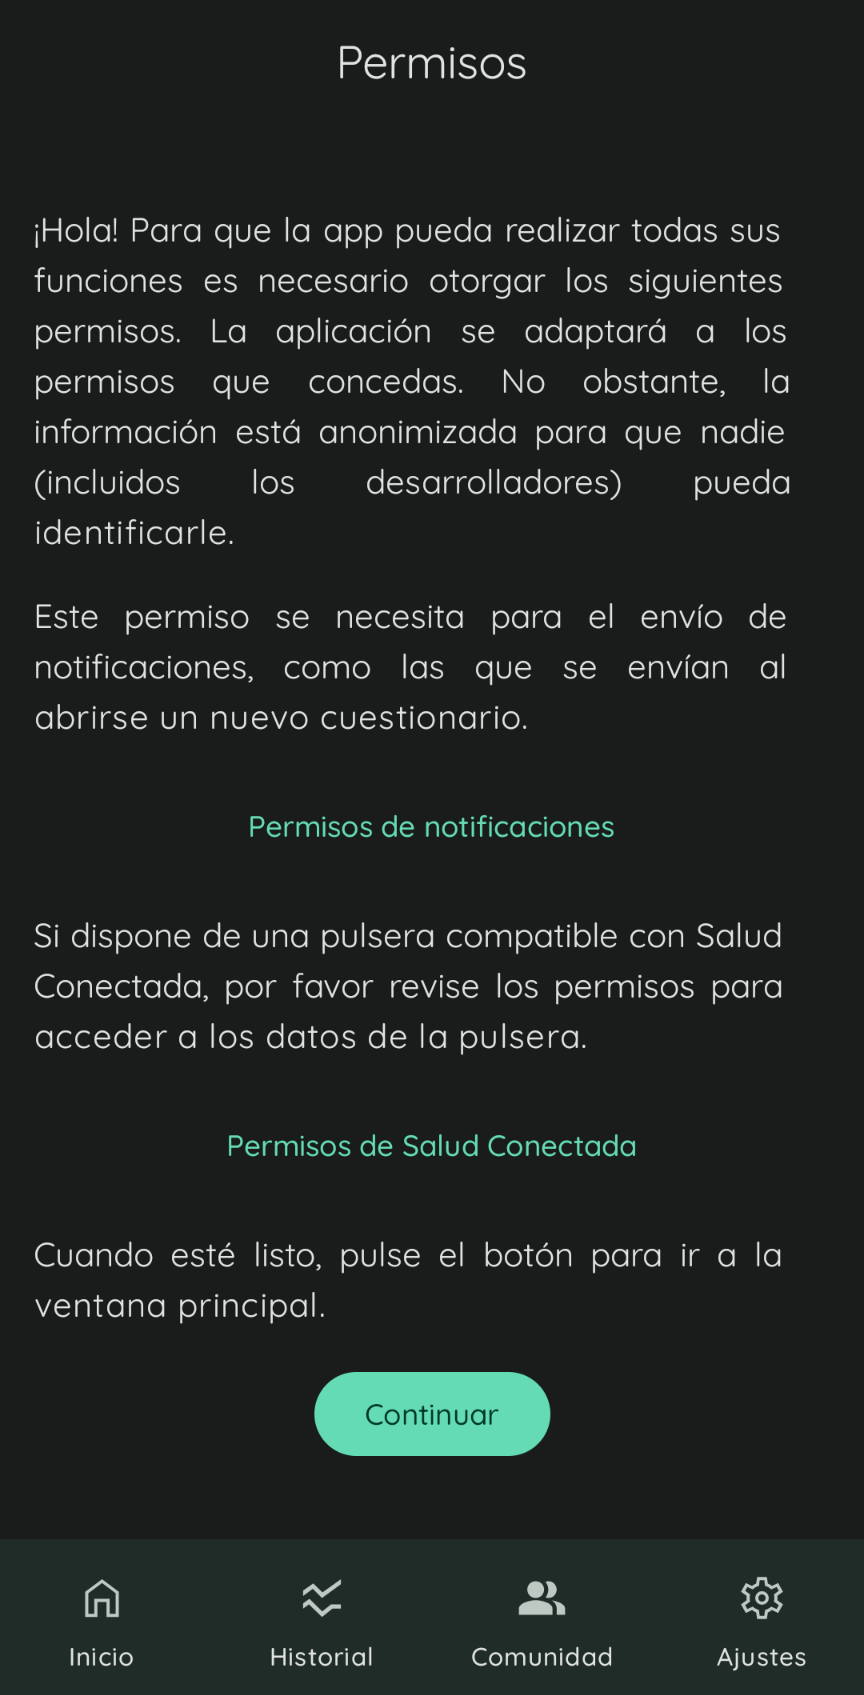
\includegraphics[width=0.4\textwidth]{figures/pantallas/Permisos.png}
                	\caption{Pantalla permisos}
                	\label{figure:implementacion:pantalla:permisos}
                \end{figure}
                
                \clearpage  % Asegura que todas las figuras y tablas pendientes se impriman antes de continuar.
            \subsubsection*{Inicio}

                Esta ventana es una de las ventanas principales de la aplicación y presenta al usuario el último estado sobre estrés, soledad o depresión en forma de carrousel. 
                
                La representación de la medida cuenta con un indicador circular que muestra qué tan grave es la medida, información sobre el nivel en cuestión y los accesos al consejo ofrecido y a la ventana \textit{medida} para obtener más información.

                En el caso que el usuario tenga cuestionarios pendientes se mostrará un aviso que el usuario podrá cerrar en cualquier momento.

                La Figura \ref{figure:implementacion:pantalla:inicio} muestra la pantalla para un caso habitual y un caso donde el último cuestionario no fue realizado.

                \begin{figure}[htbp]
                	\centering
                	\begin{subfigure}[c]{0.4\textwidth}
                		\centering
                		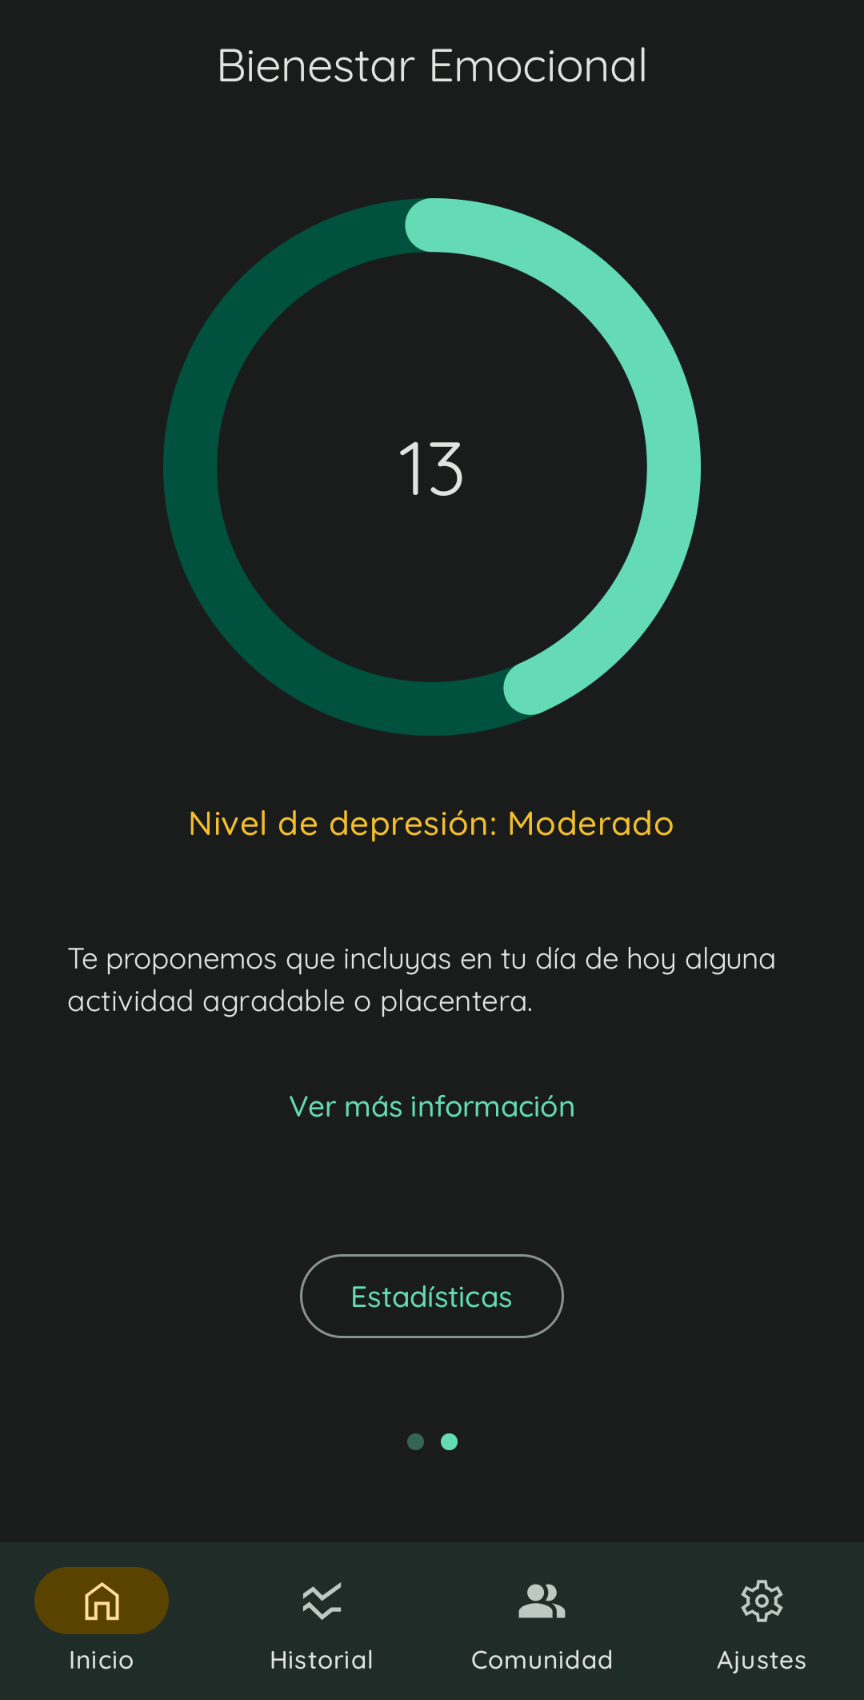
\includegraphics[width=1\textwidth]{figures/pantallas/Inicio.png}
                	\end{subfigure}
                	\hspace{0.1\textwidth}
                	\begin{subfigure}[c]{0.4\textwidth}
                		\centering
                		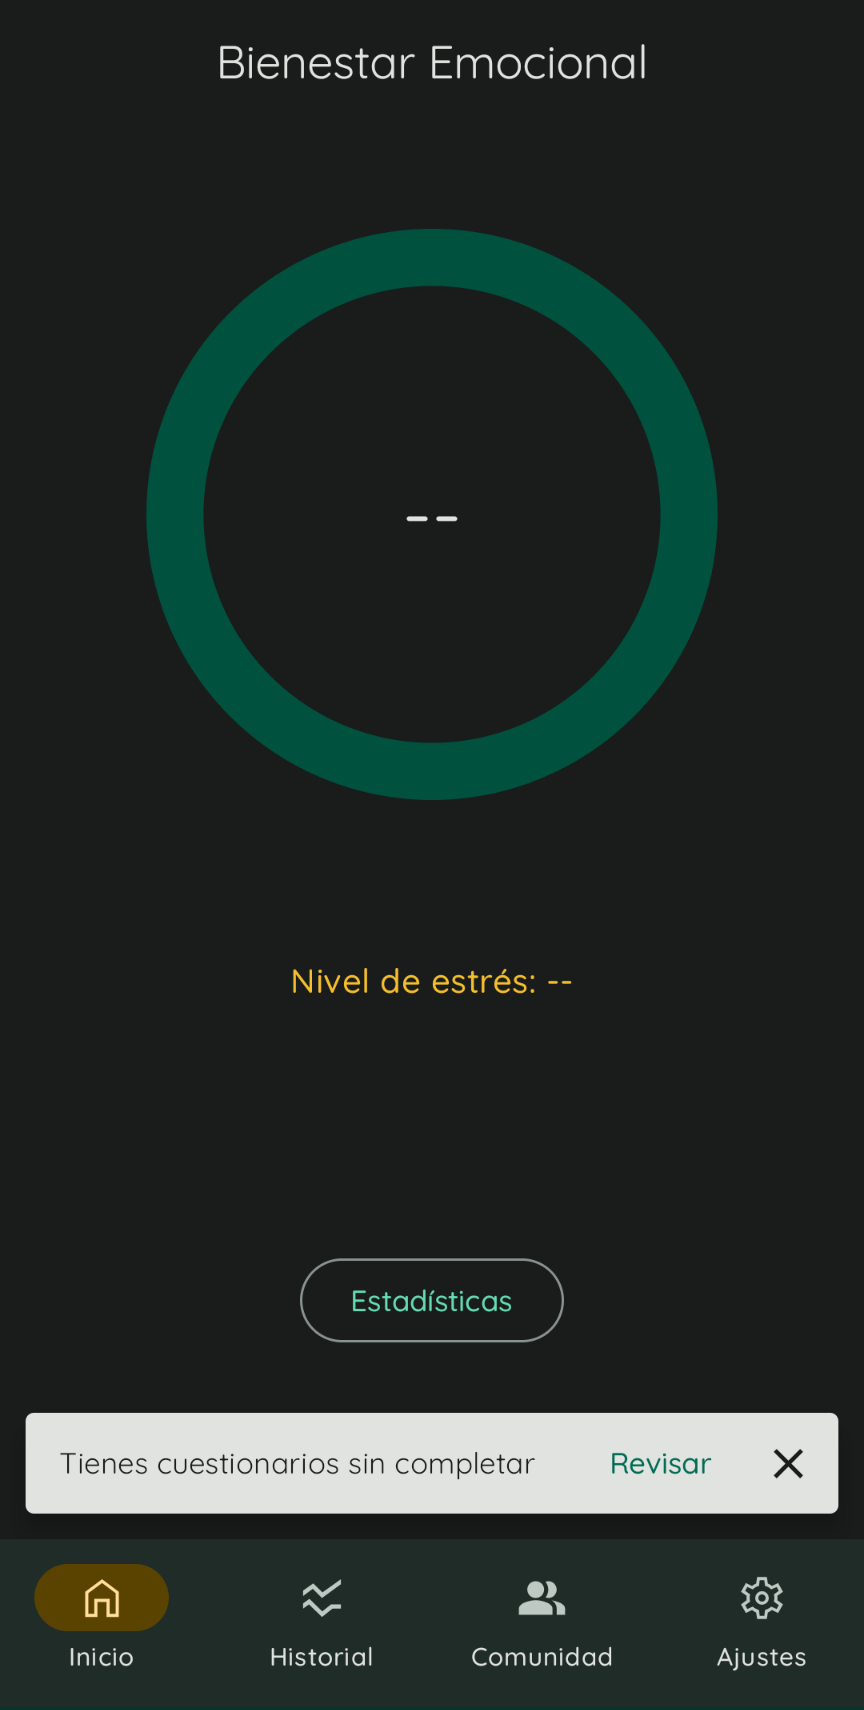
\includegraphics[width=1\linewidth]{figures/pantallas/Inicio con pendientes.png}
                	\end{subfigure}
                	\caption{Pantalla inicio}
                	\label{figure:implementacion:pantalla:inicio}
                \end{figure}
                
                \clearpage  % Asegura que todas las figuras y tablas pendientes se impriman antes de continuar.
            \subsubsection*{Historial}
                Esta ventana es otra de las principales e implementa la visualización de estadísticas acerca del historial del usuario. Los ajustes de medida y granularidad se han implementado mediante desplegables, mientras que el ajuste de la fecha se realiza mediante un diálogo.

                Por otra parte, la estadística se trata de un diagrama de líneas estableciéndose un marcador en la medida de cada día, etiquetándose los eje x e y con la granularidad y el nivel de la medida respectivamente.
                
                La Figura \ref{figure:implementacion:pantalla:historial} muestra esta pantalla en acción.
                
                \begin{figure}[h]
                	\centering
                	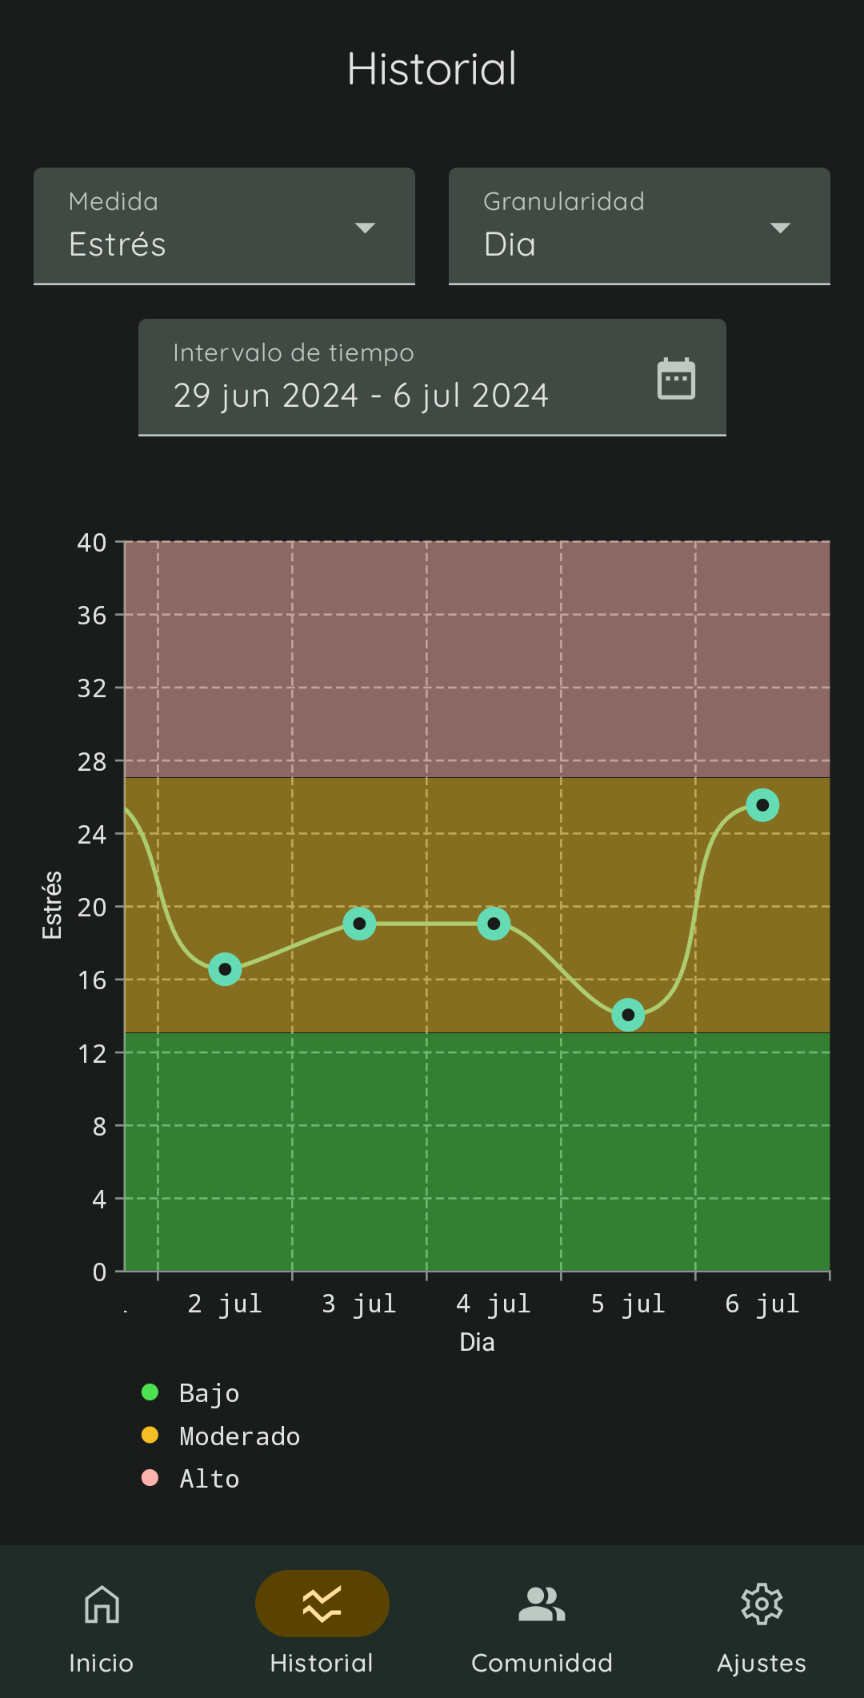
\includegraphics[width=0.4\textwidth]{figures/pantallas/Historial.png}
                	\caption{Pantalla historial}
                	\label{figure:implementacion:pantalla:historial}
                \end{figure}
                
                \clearpage  % Asegura que todas las figuras y tablas pendientes se impriman antes de continuar.
            \subsubsection*{Comunidad}
                
                La tercera de las ventanas principales implementa la funcionalidad de seguimiento conjunto, nuevamente en forma de carrousel para que el usuario pueda moverse entre medidas.

                En cuanto a la representación gráfica se han elegido dos indicadores circulares, que a diferencia de los anteriores, muestran el nivel de la medida dentro del círculo. 
                
                Más abajo se encuentra el diagrama de barras que representa la semana actual para la comunidad, estando nuevamente los ejes x e y etiquetados, en este caso con los días de la semana y el nivel de la medida respectivamente.

                La Figura \ref{figure:implementacion:pantalla:comunidad} representa esta pantalla.
                
                \begin{figure}[h]
                	\centering
                	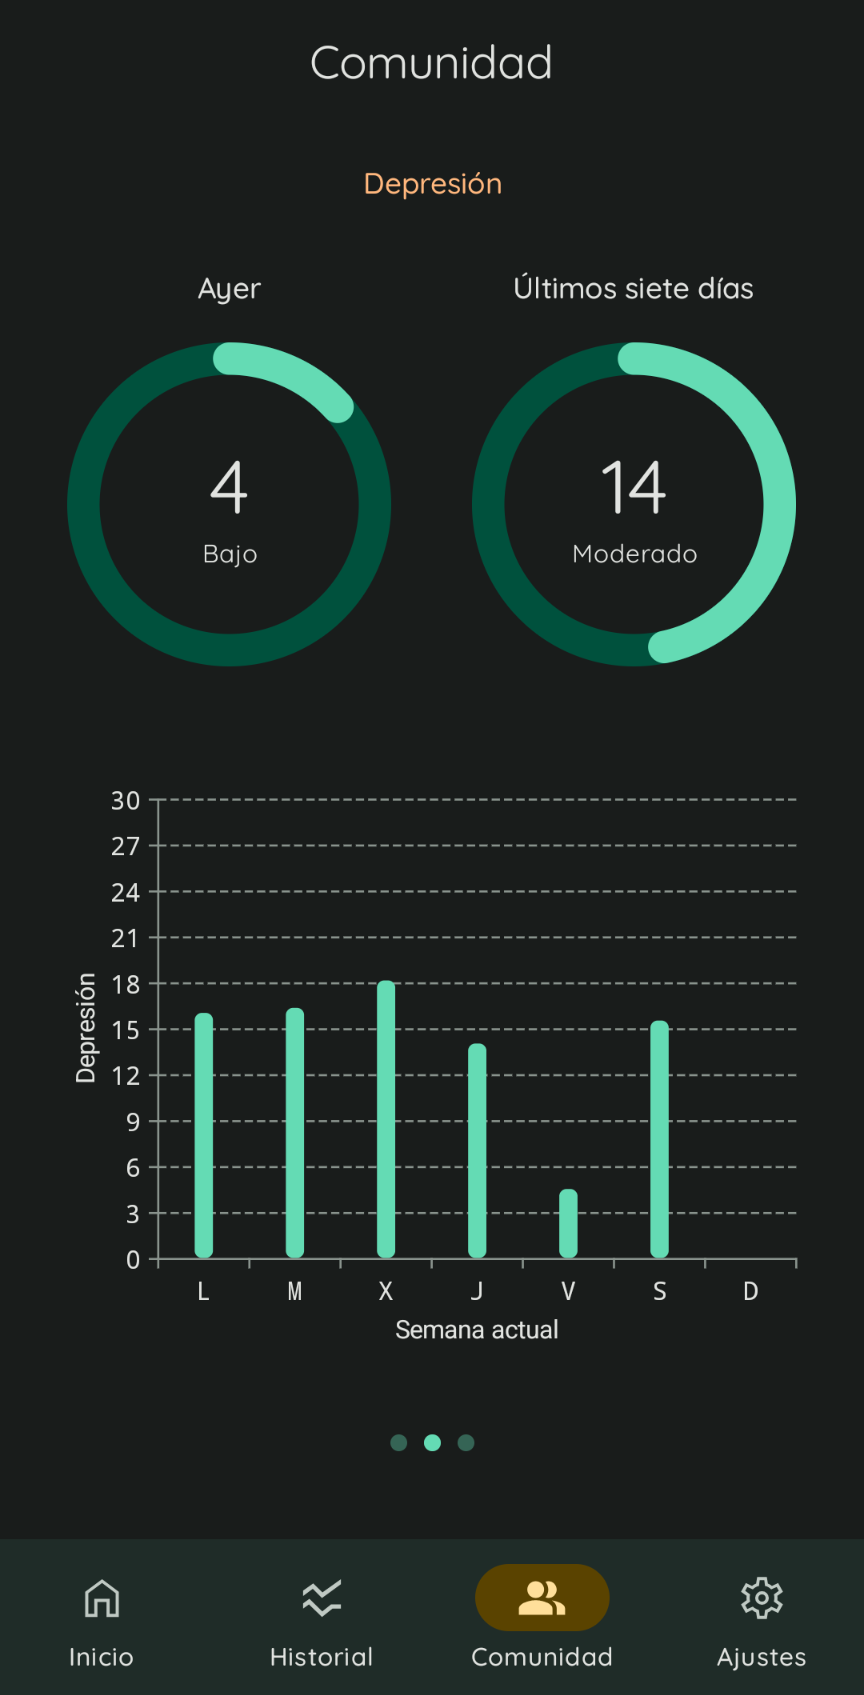
\includegraphics[width=0.4\textwidth]{figures/pantallas/Comunidad.png}
                	\caption{Pantalla comunidad}
                	\label{figure:implementacion:pantalla:comunidad}
                \end{figure}
                
                \clearpage  % Asegura que todas las figuras y tablas pendientes se impriman antes de continuar.
            \subsubsection*{Ajustes}

                La cuarta y última ventana principal consta de un amplio abanico de funciones y accesos a otras ventanas. La Figura \ref{figure:implementacion:pantalla:ajustes} muestra el contenido de esta pantalla en su conjunto.
                
                \begin{figure}[htbp]
                	\centering
                	\begin{subfigure}[c]{0.29\textwidth}
                		\centering
                		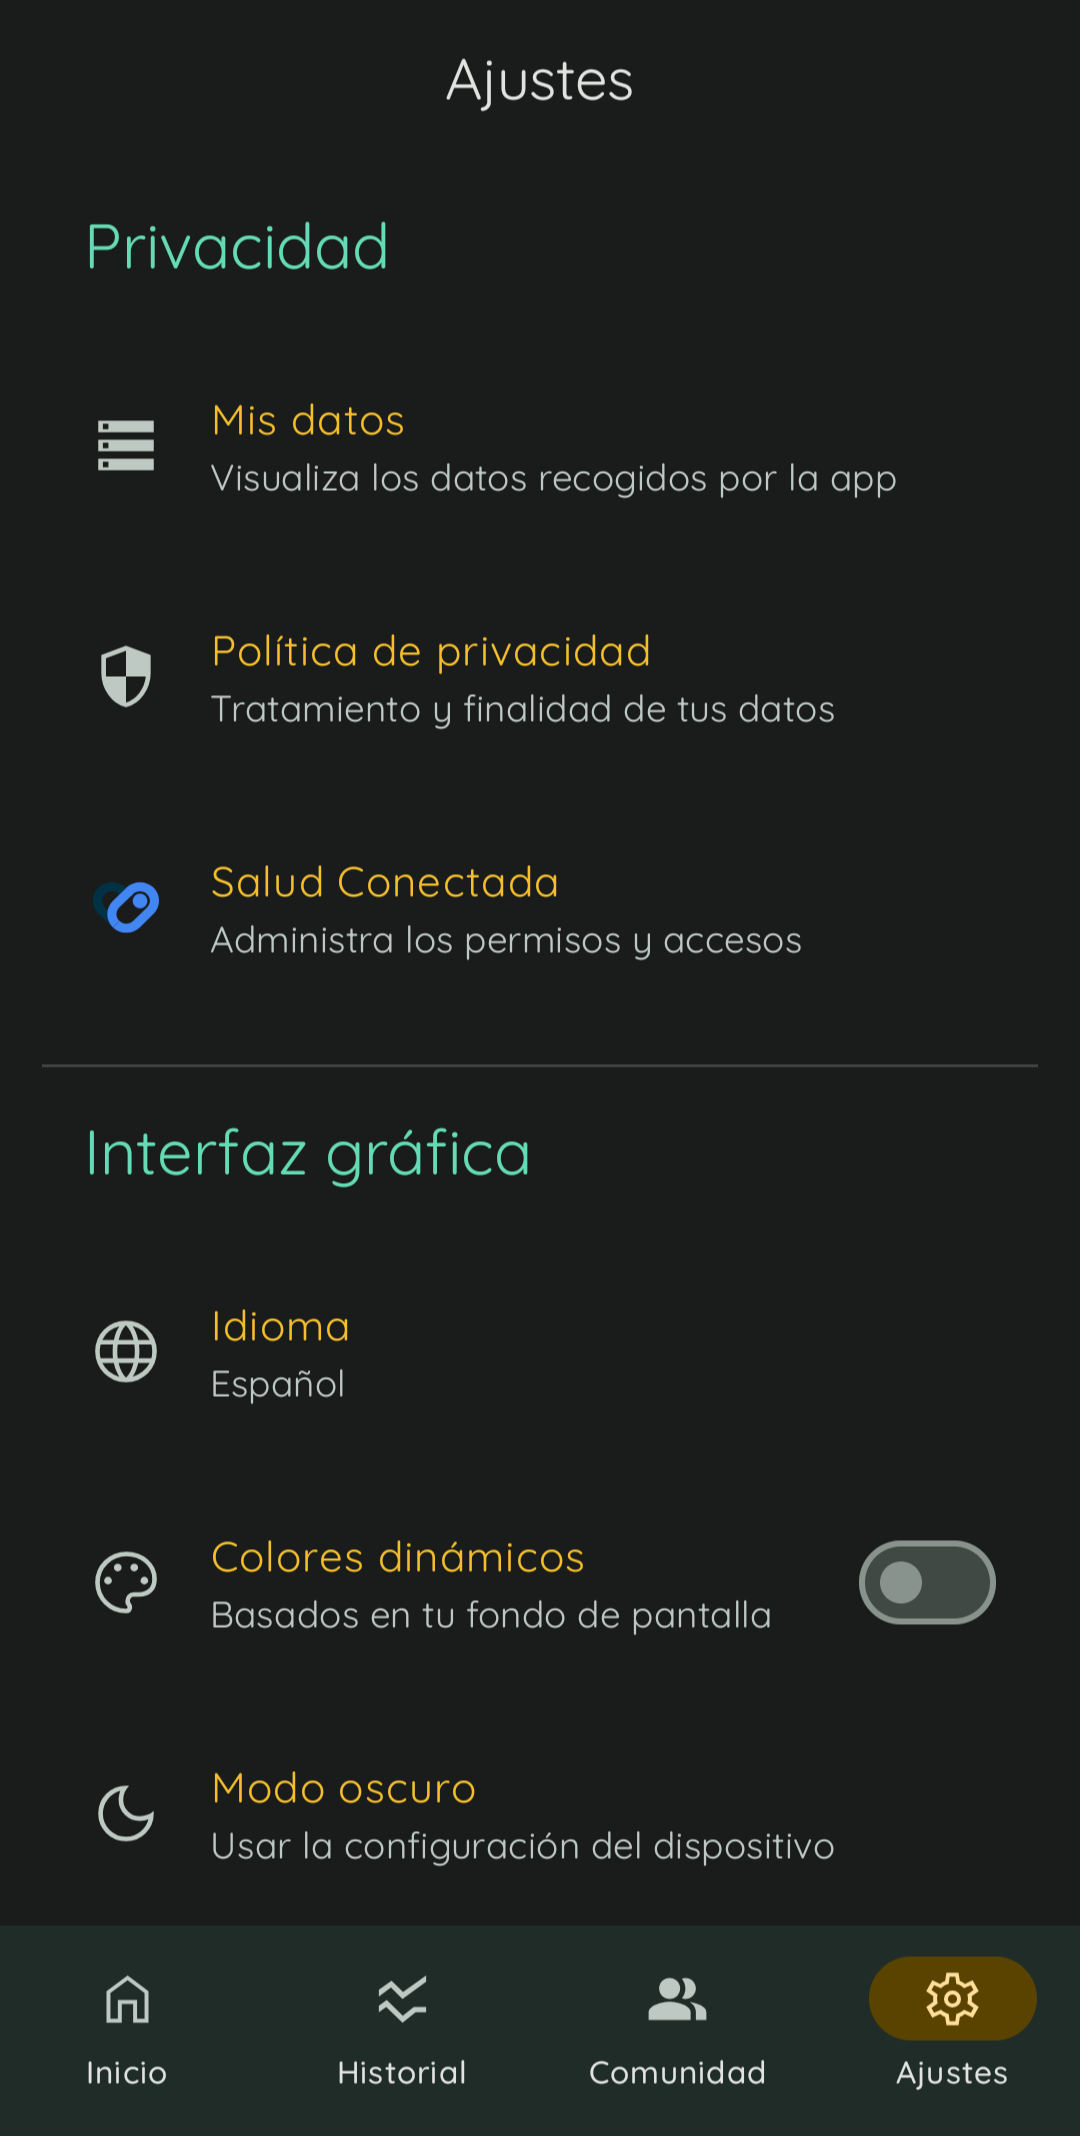
\includegraphics[width=1\textwidth]{figures/pantallas/Ajustes 1.png}
                	\end{subfigure}
                	\hspace{0.05\textwidth}
                	\begin{subfigure}[c]{0.29\textwidth}
                		\centering
                		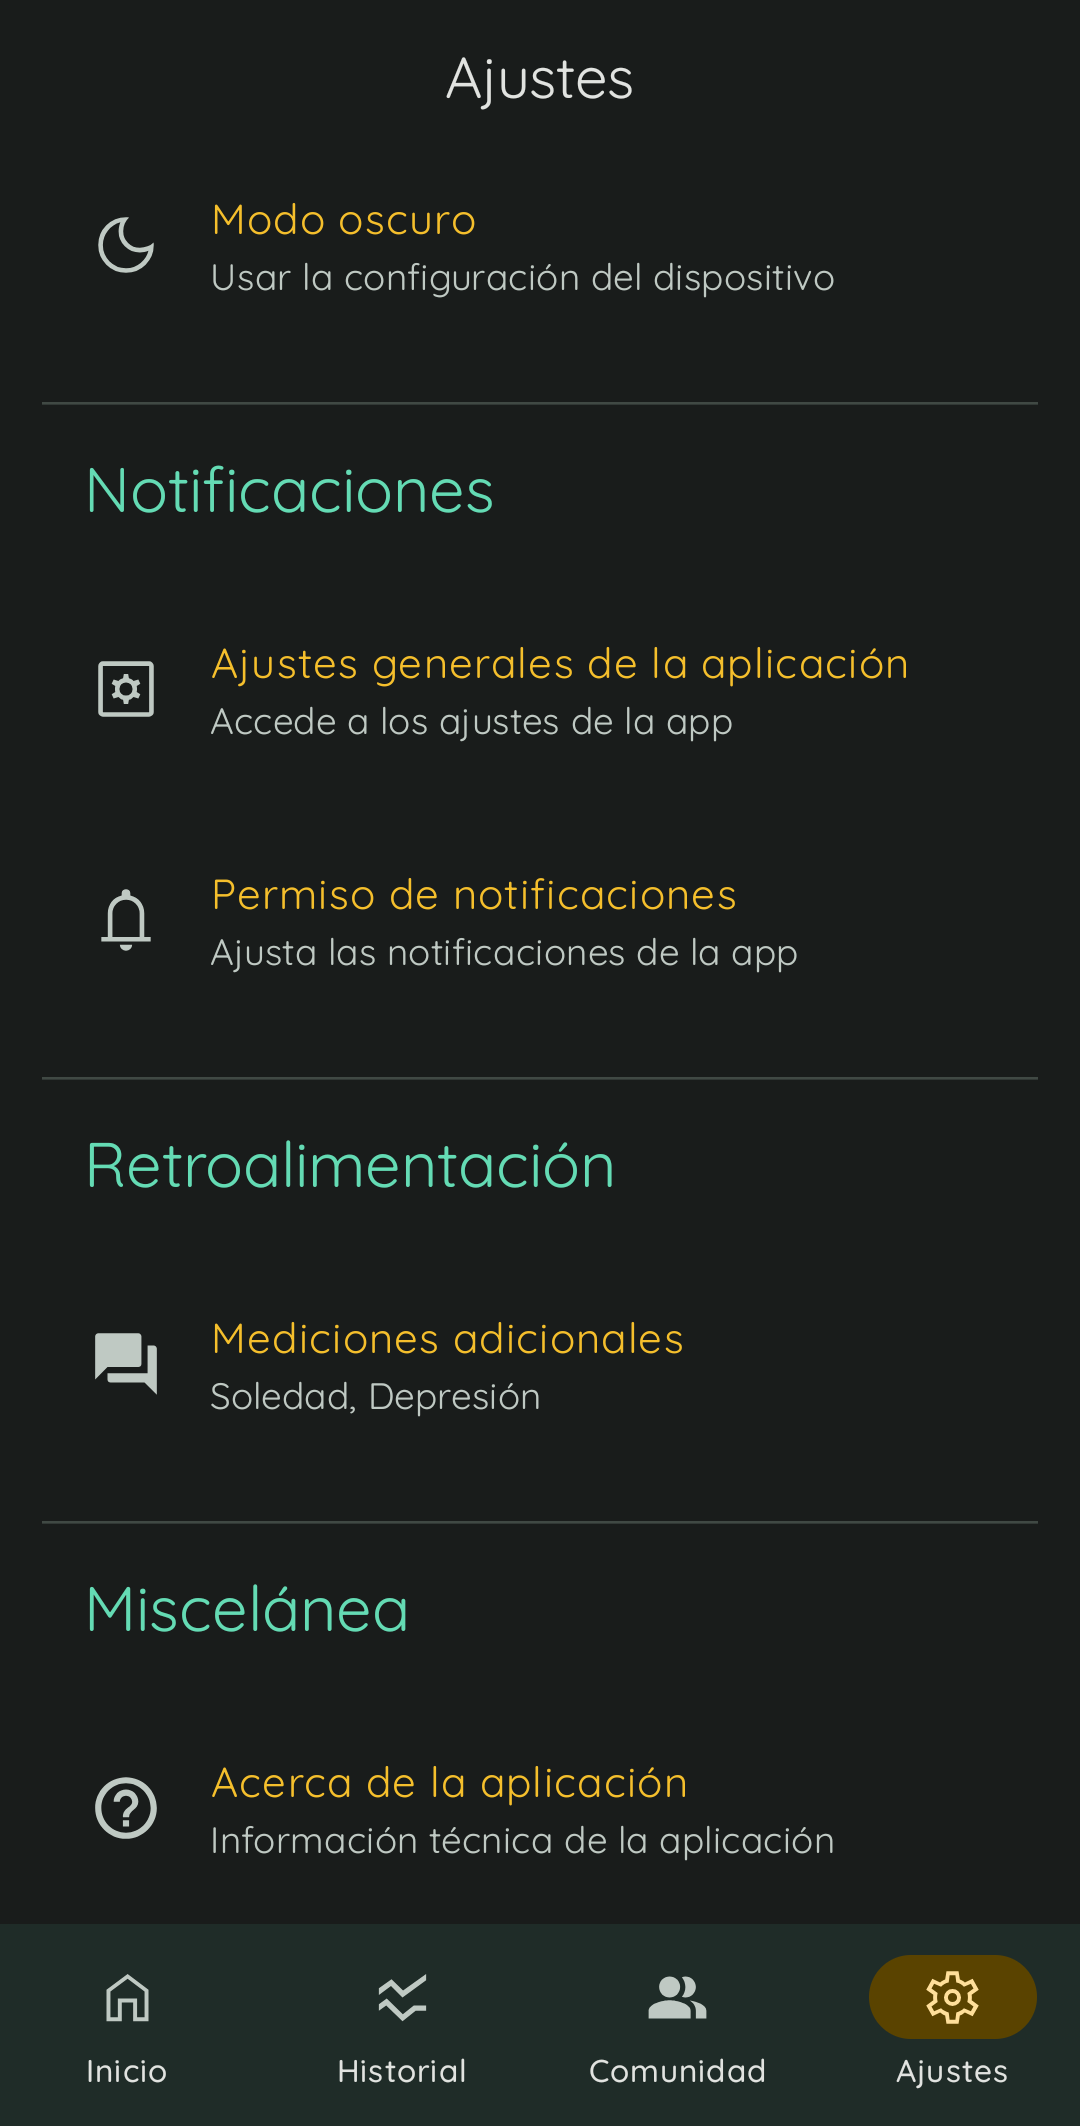
\includegraphics[width=1\linewidth]{figures/pantallas/Ajustes 2.png}
                	\end{subfigure}
                    \hspace{0.05\textwidth}
                	\begin{subfigure}[c]{0.29\textwidth}
                		\centering
                		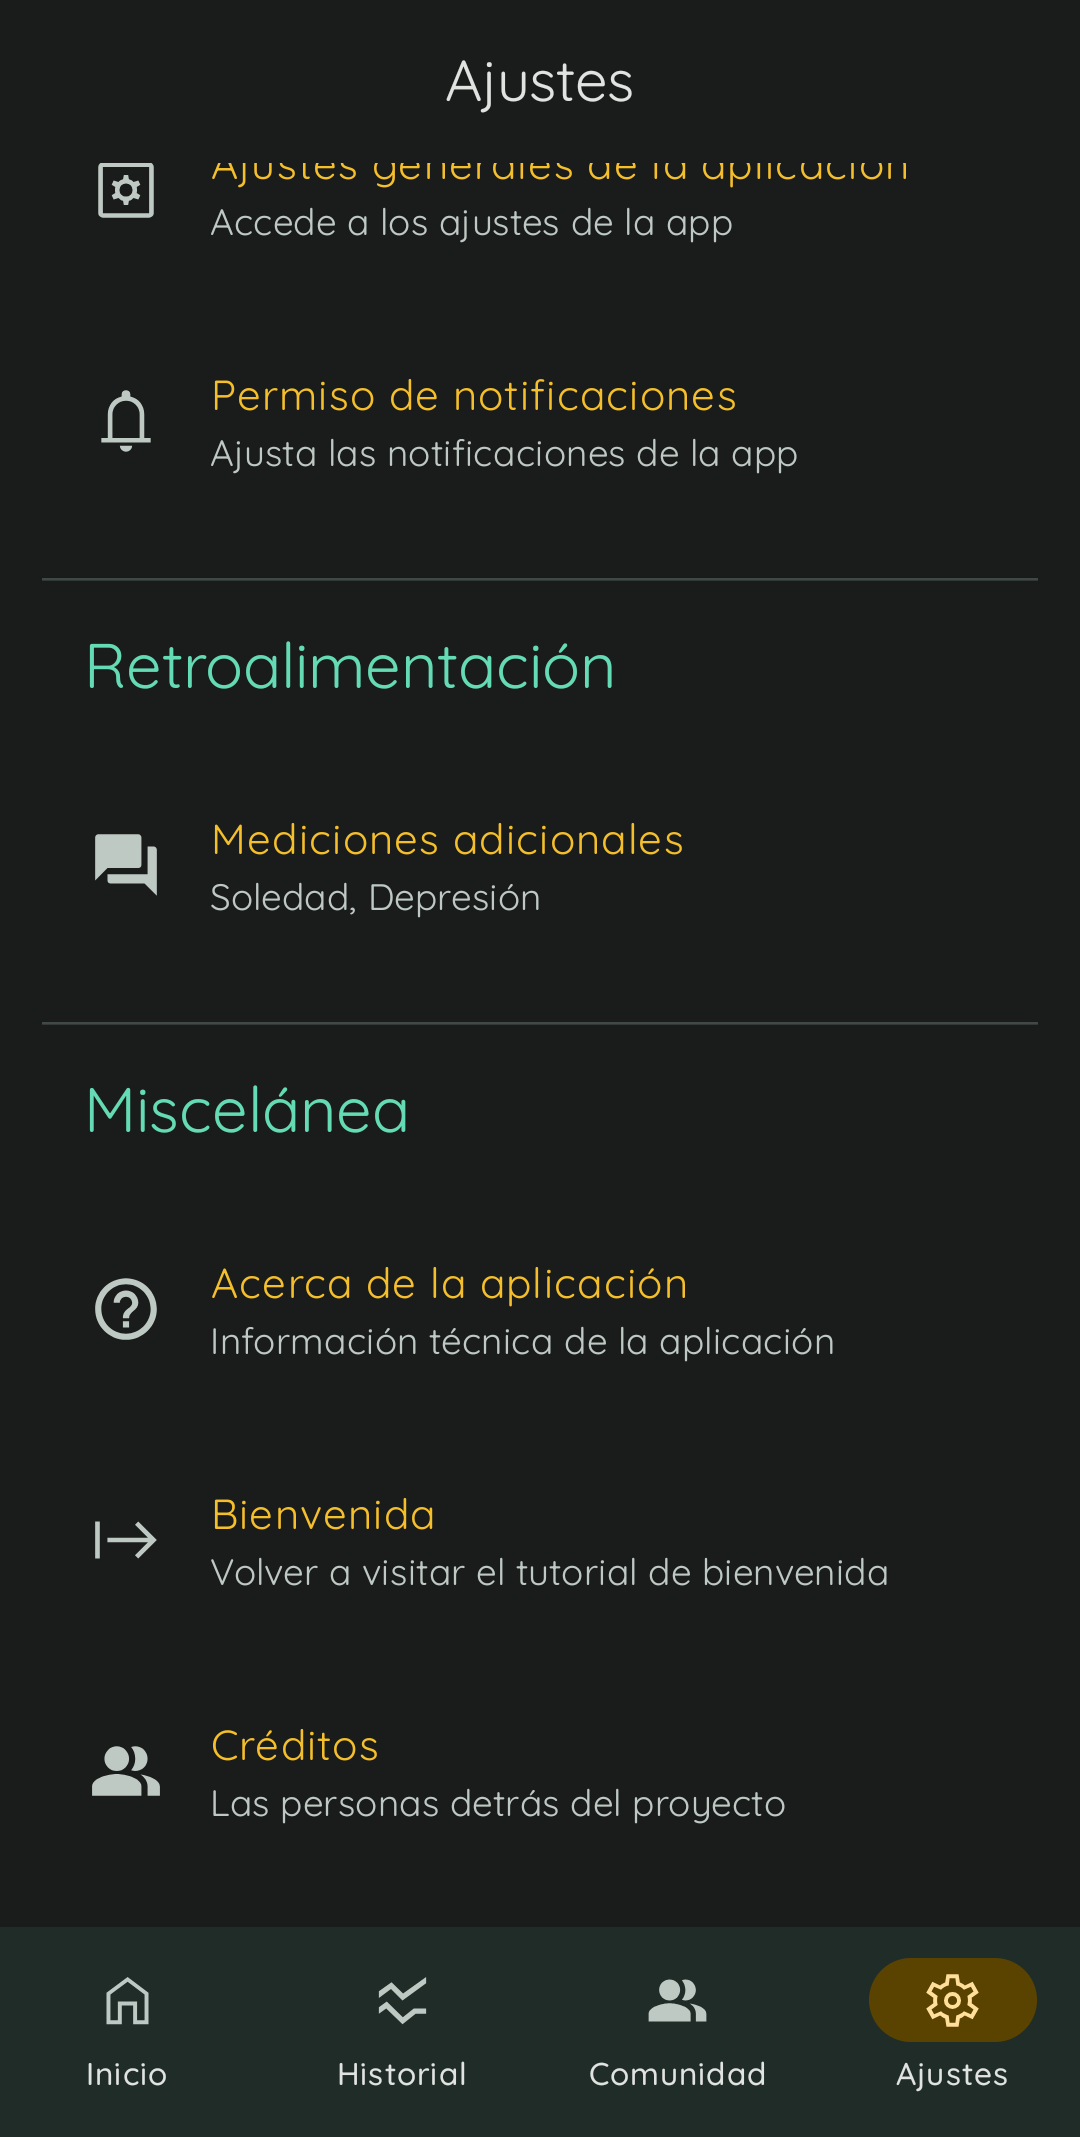
\includegraphics[width=1\linewidth]{figures/pantallas/Ajustes 3.png}
                	\end{subfigure}
                	\caption{Pantalla ajustes}
                	\label{figure:implementacion:pantalla:ajustes}
                \end{figure}

                Por otra parte la Figura \ref{figure:implementacion:pantalla:paneles_ajustes} representa los paneles de Android que se pueden abrir desde ajustes.
                
                \begin{figure}[htbp]
                	\centering
                	\begin{subfigure}[c]{0.29\textwidth}
                		\centering
                		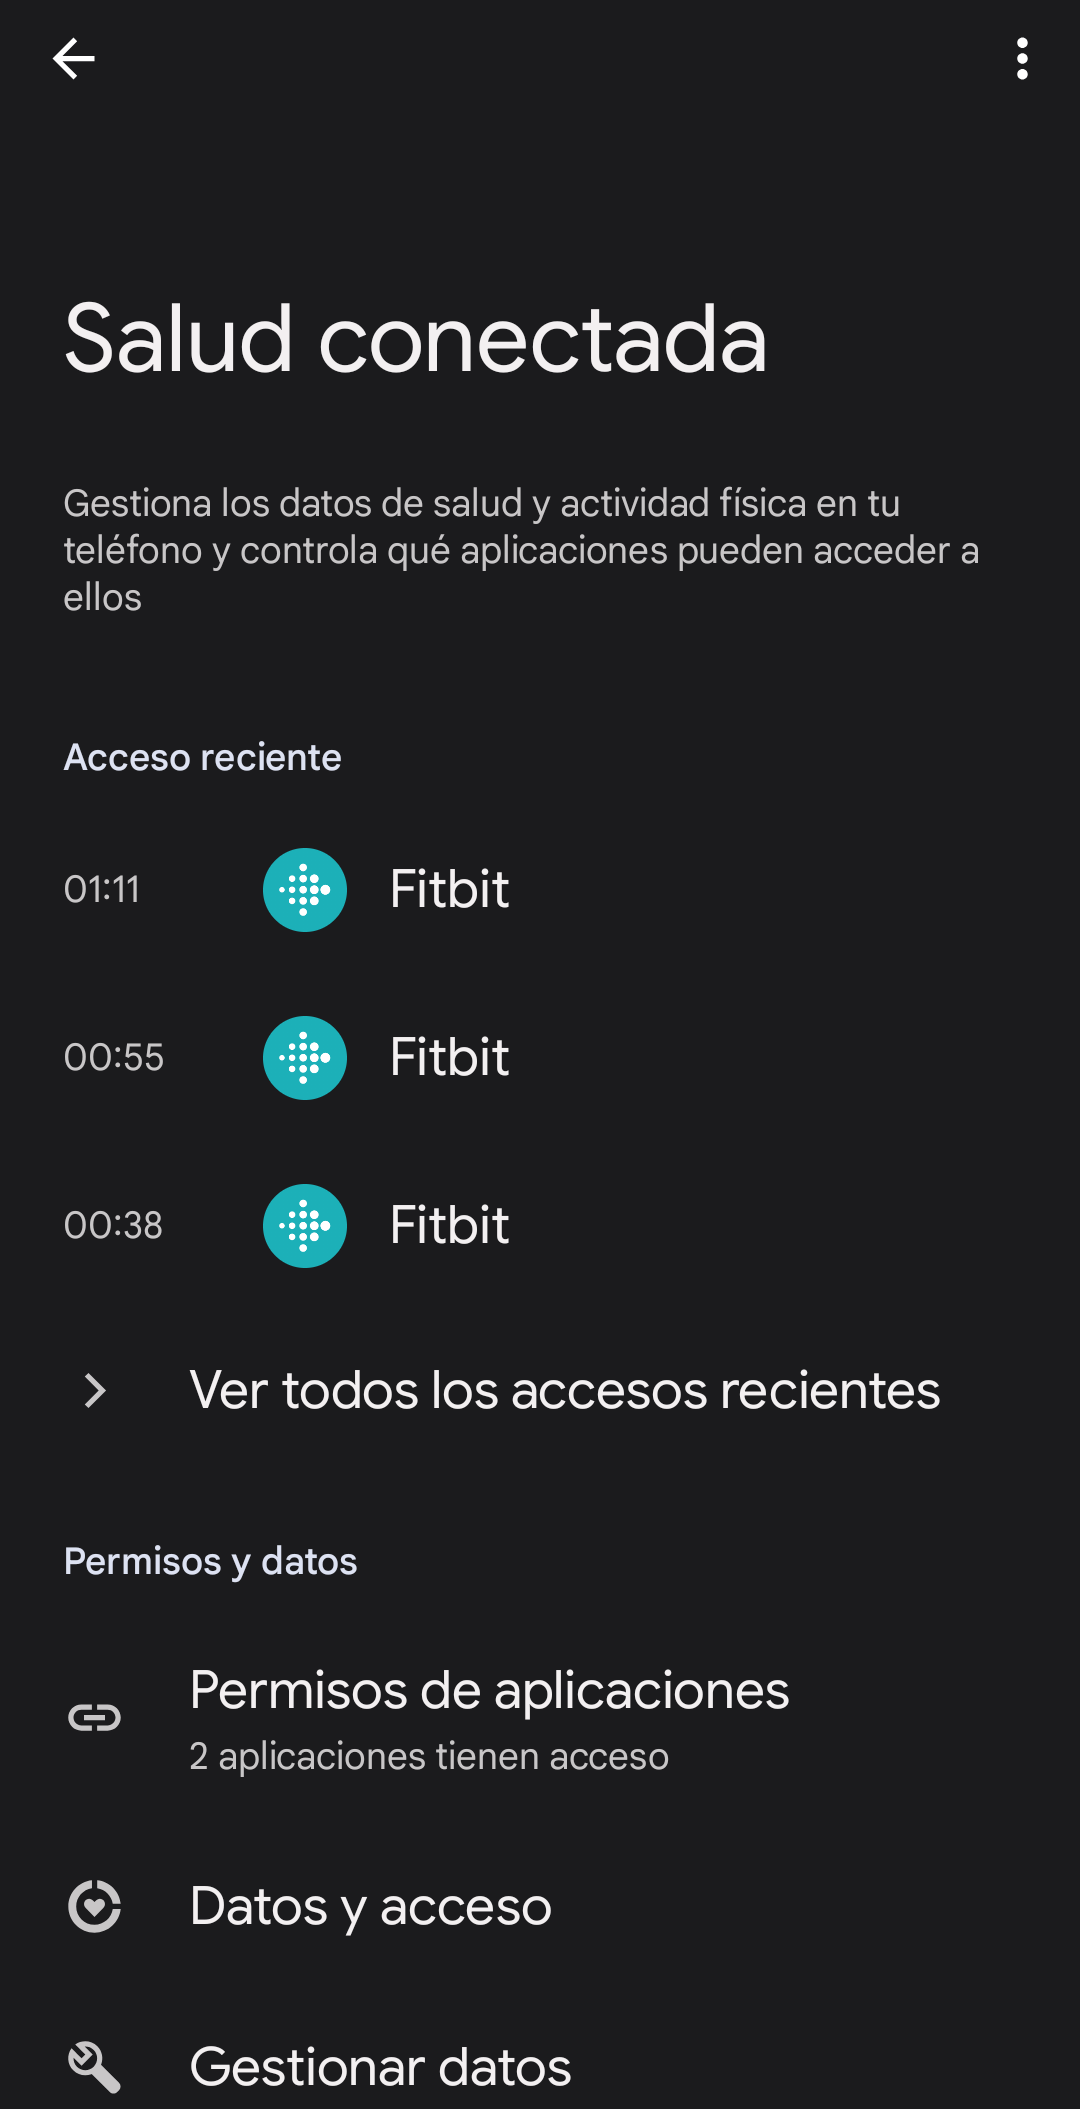
\includegraphics[width=1\textwidth]{figures/pantallas/Salud Conectada.png}
                	\end{subfigure}
                	\hspace{0.05\textwidth}
                	\begin{subfigure}[c]{0.29\textwidth}
                		\centering
                		\includegraphics[width=1\linewidth]{figures/pantallas/Información app.png}
                	\end{subfigure}
                    \hspace{0.05\textwidth}
                	\begin{subfigure}[c]{0.29\textwidth}
                		\centering
                		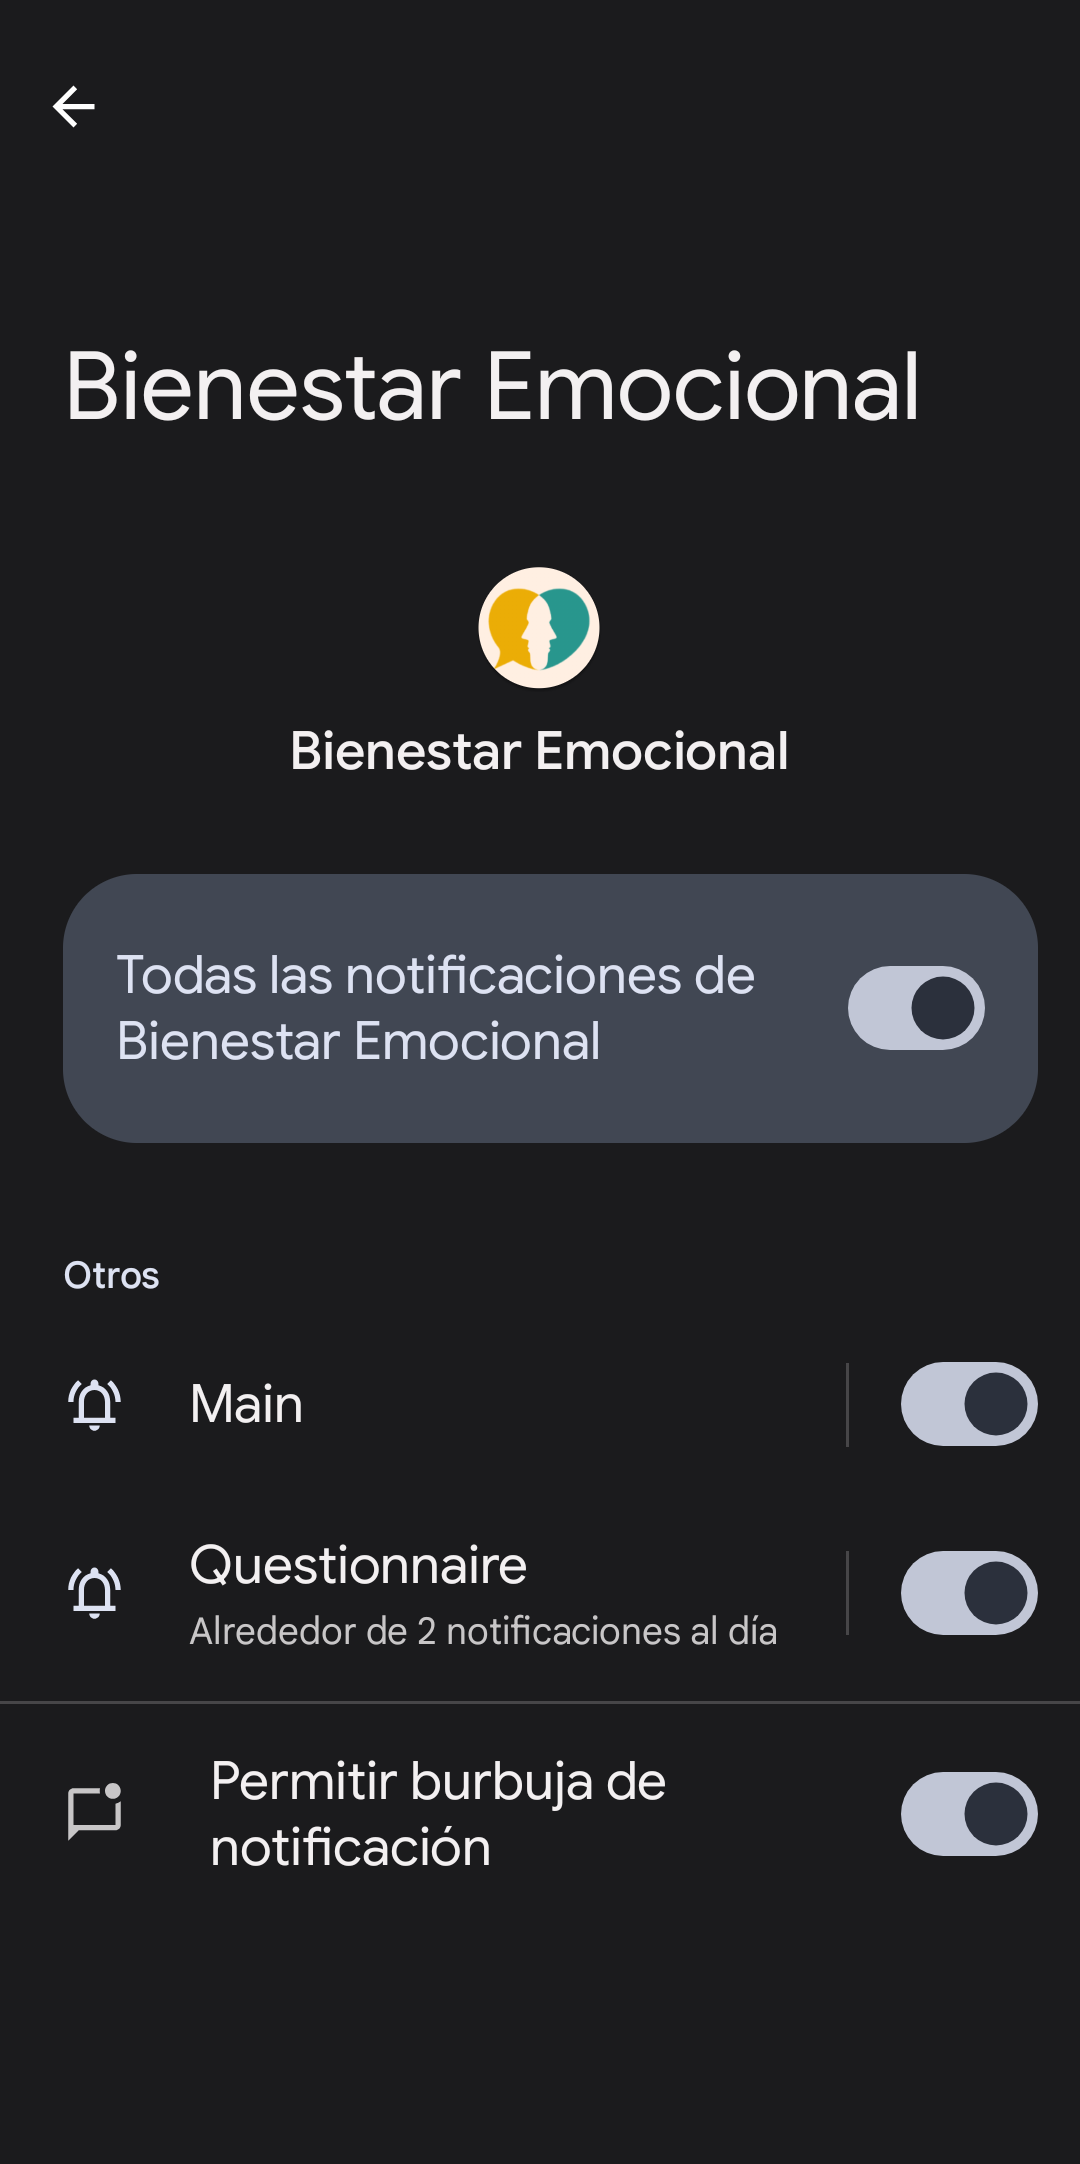
\includegraphics[width=1\linewidth]{figures/pantallas/Permiso notificaciones.png}
                	\end{subfigure}
                	\caption{Paneles accesibles desde ajustes}
                	\label{figure:implementacion:pantalla:paneles_ajustes}
                \end{figure}

                Por último, la Figura \ref{figure:implementacion:pantalla:dialogos_ajustes} muestra la implementación de los diálogos de idioma, modo y mediciones respectivamente.

                \begin{figure}[htbp]
                	\centering
                	\begin{subfigure}[c]{0.29\textwidth}
                		\centering
                		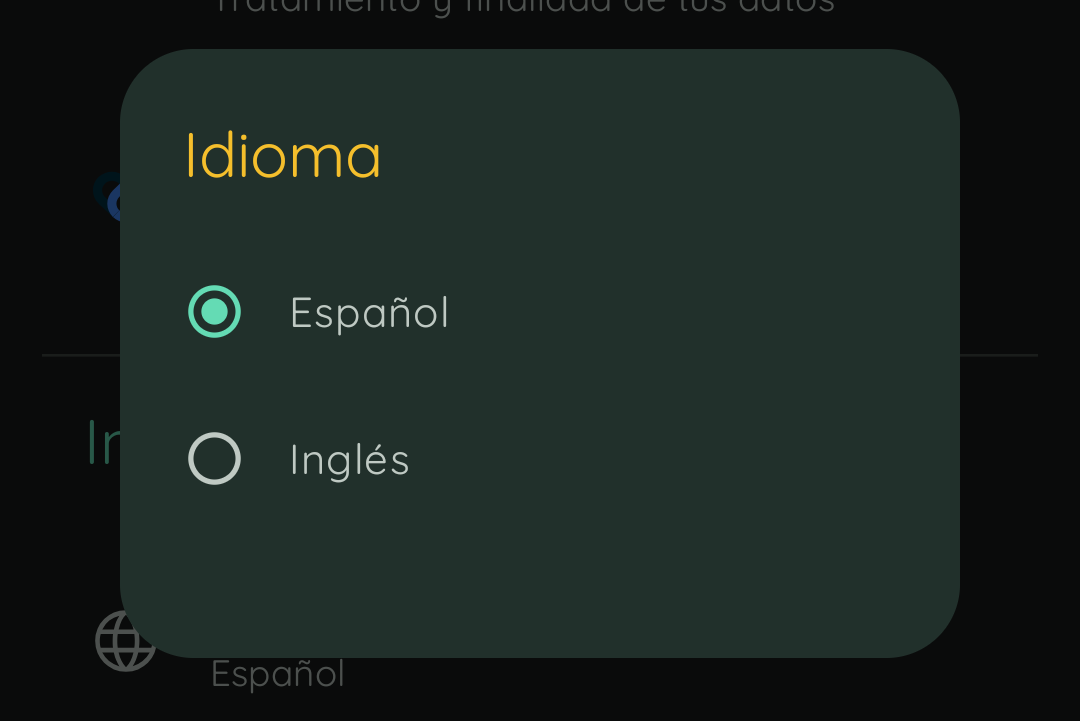
\includegraphics[width=1\textwidth]{figures/pantallas/Ajuste idioma.png}
                	\end{subfigure}
                	\hspace{0.05\textwidth}
                	\begin{subfigure}[c]{0.29\textwidth}
                		\centering
                		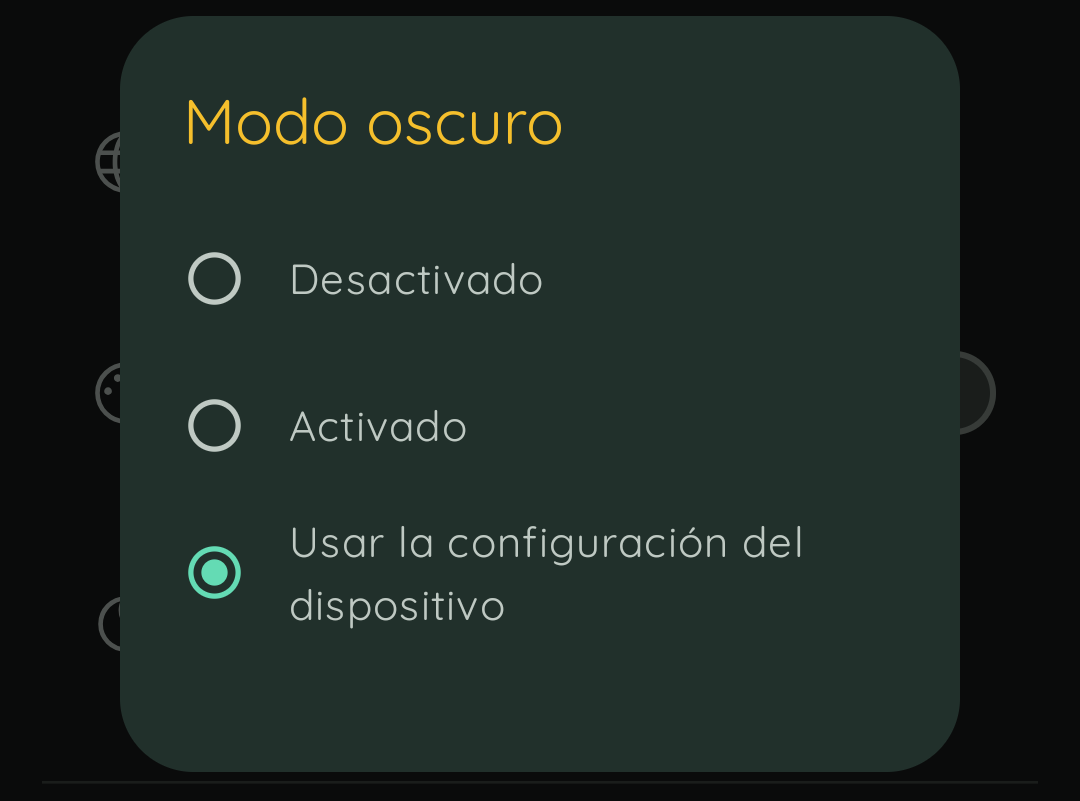
\includegraphics[width=1\linewidth]{figures/pantallas/Ajuste modo.png}
                	\end{subfigure}
                    \hspace{0.05\textwidth}
                	\begin{subfigure}[c]{0.29\textwidth}
                		\centering
                		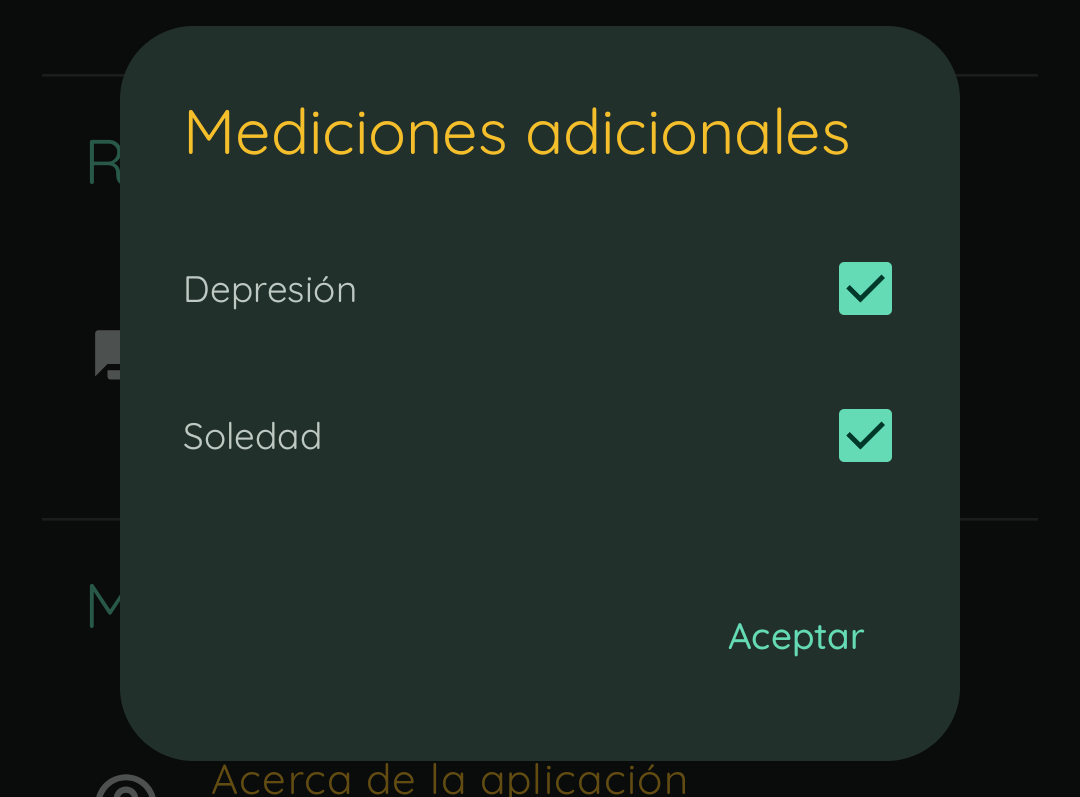
\includegraphics[width=1\linewidth]{figures/pantallas/Ajuste mediciones.png}
                	\end{subfigure}
                	\caption{Diálogos de ajustes}
                	\label{figure:implementacion:pantalla:dialogos_ajustes}
                \end{figure}
                
                \clearpage  % Asegura que todas las figuras y tablas pendientes se impriman antes de continuar.
            \subsubsection*{Consejo}

                Esta pantalla consta únicamente del texto detallado del consejo y de un botón para volver atrás. La Figura muestra la pantalla consejo ofreciendo la recomendación para mitigar el estrés alto \ref{figure:implementacion:pantalla:consejo}.
                
                \begin{figure}[h]
                	\centering
                	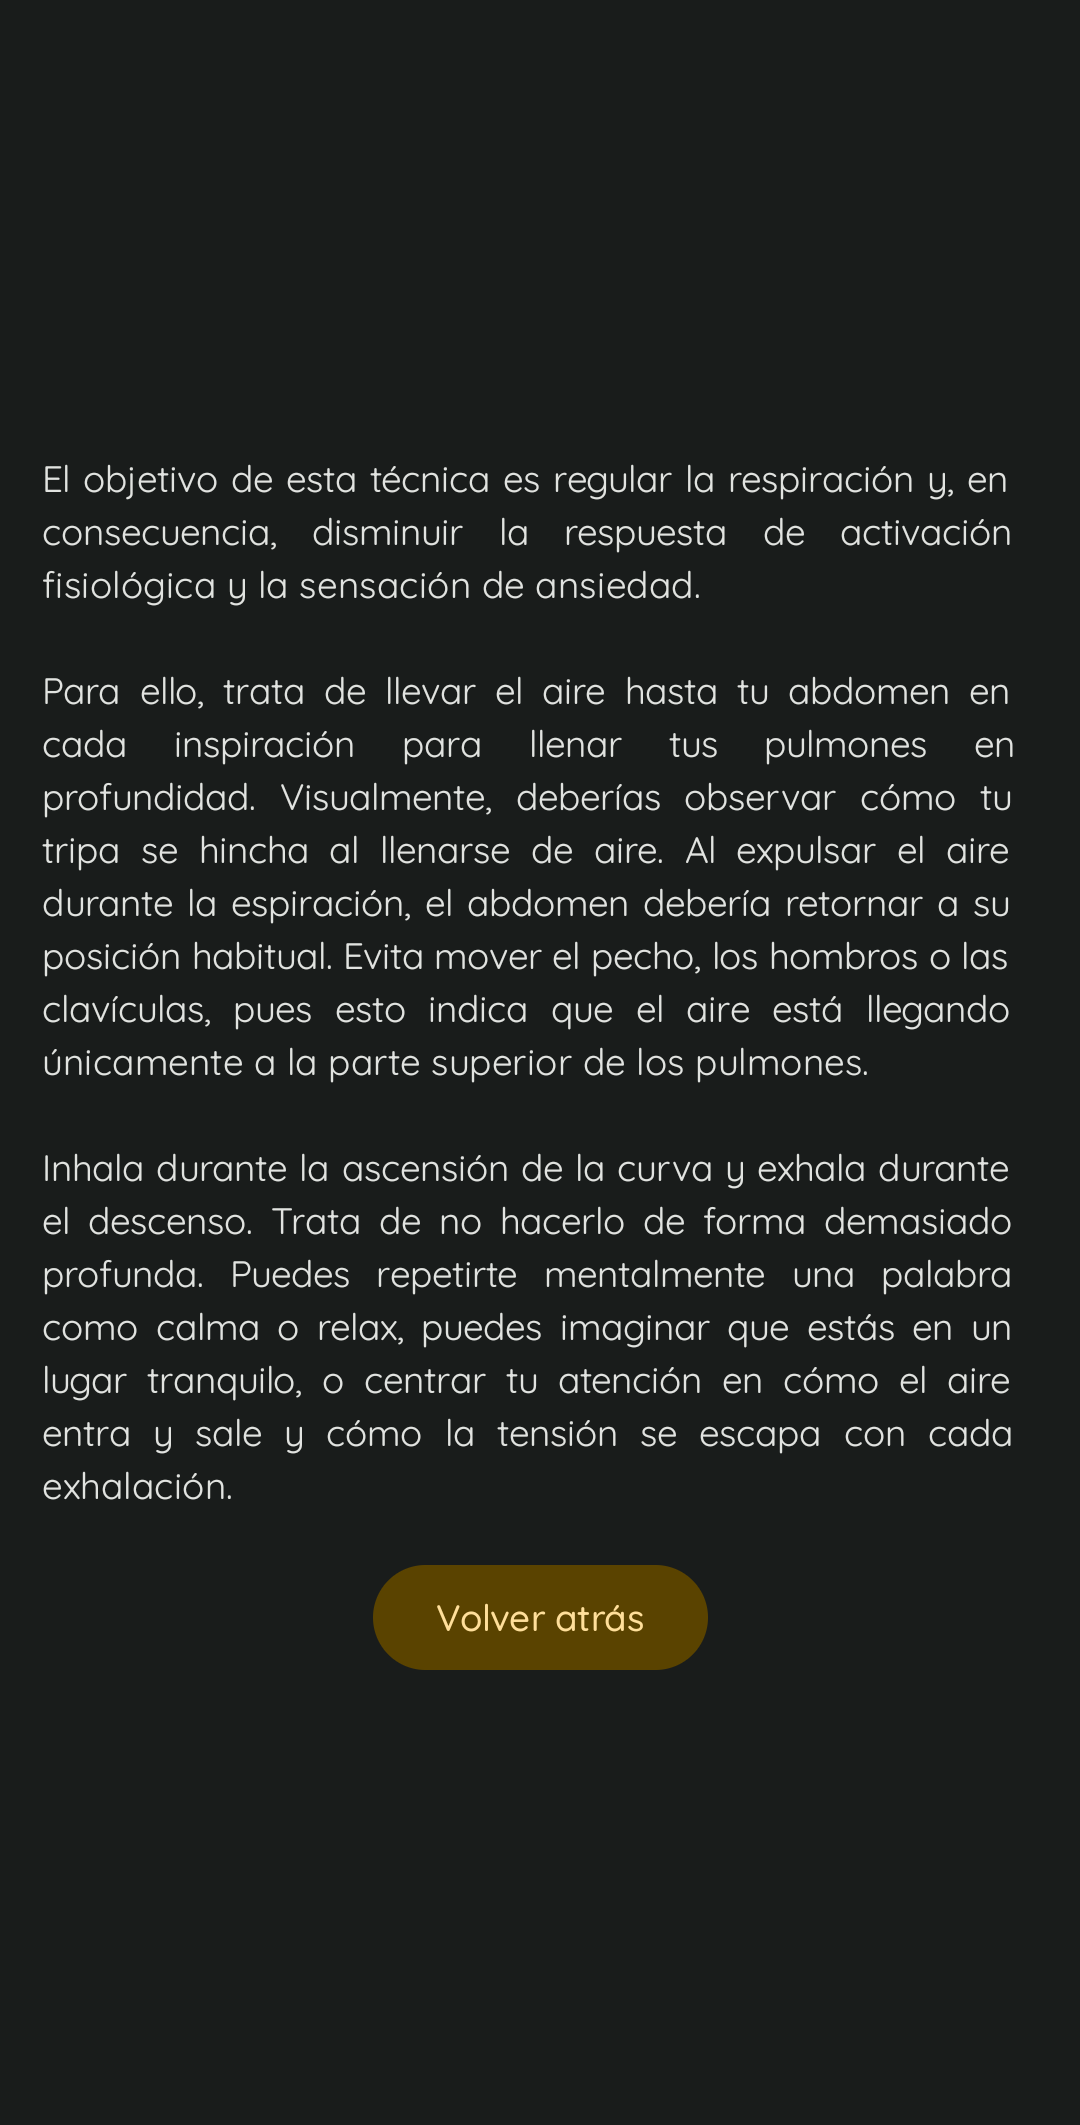
\includegraphics[width=0.4\textwidth]{figures/pantallas/Consejo estres alto.png}
                	\caption{Pantalla consejo}
                	\label{figure:implementacion:pantalla:consejo}
                \end{figure}

                \clearpage  % Asegura que todas las figuras y tablas pendientes se impriman antes de continuar.
            \subsubsection*{Medida}
                Esta pantalla básica, accesible desde inicio, consta de los mismos elementos gráficos que la ventana de comunidad con la salvedad de que son los datos del usuario los representados en esta ventana. Además consta de un botón que dirige al usuario a la pantalla de historial.

                La Figura \ref{figure:implementacion:pantalla:medida} muestra la pantalla en un caso habitual de uso y en el escenario de encontrar valores nulos.
                
                \begin{figure}[htbp]
                	\centering
                	\begin{subfigure}[c]{0.4\textwidth}
                		\centering
                		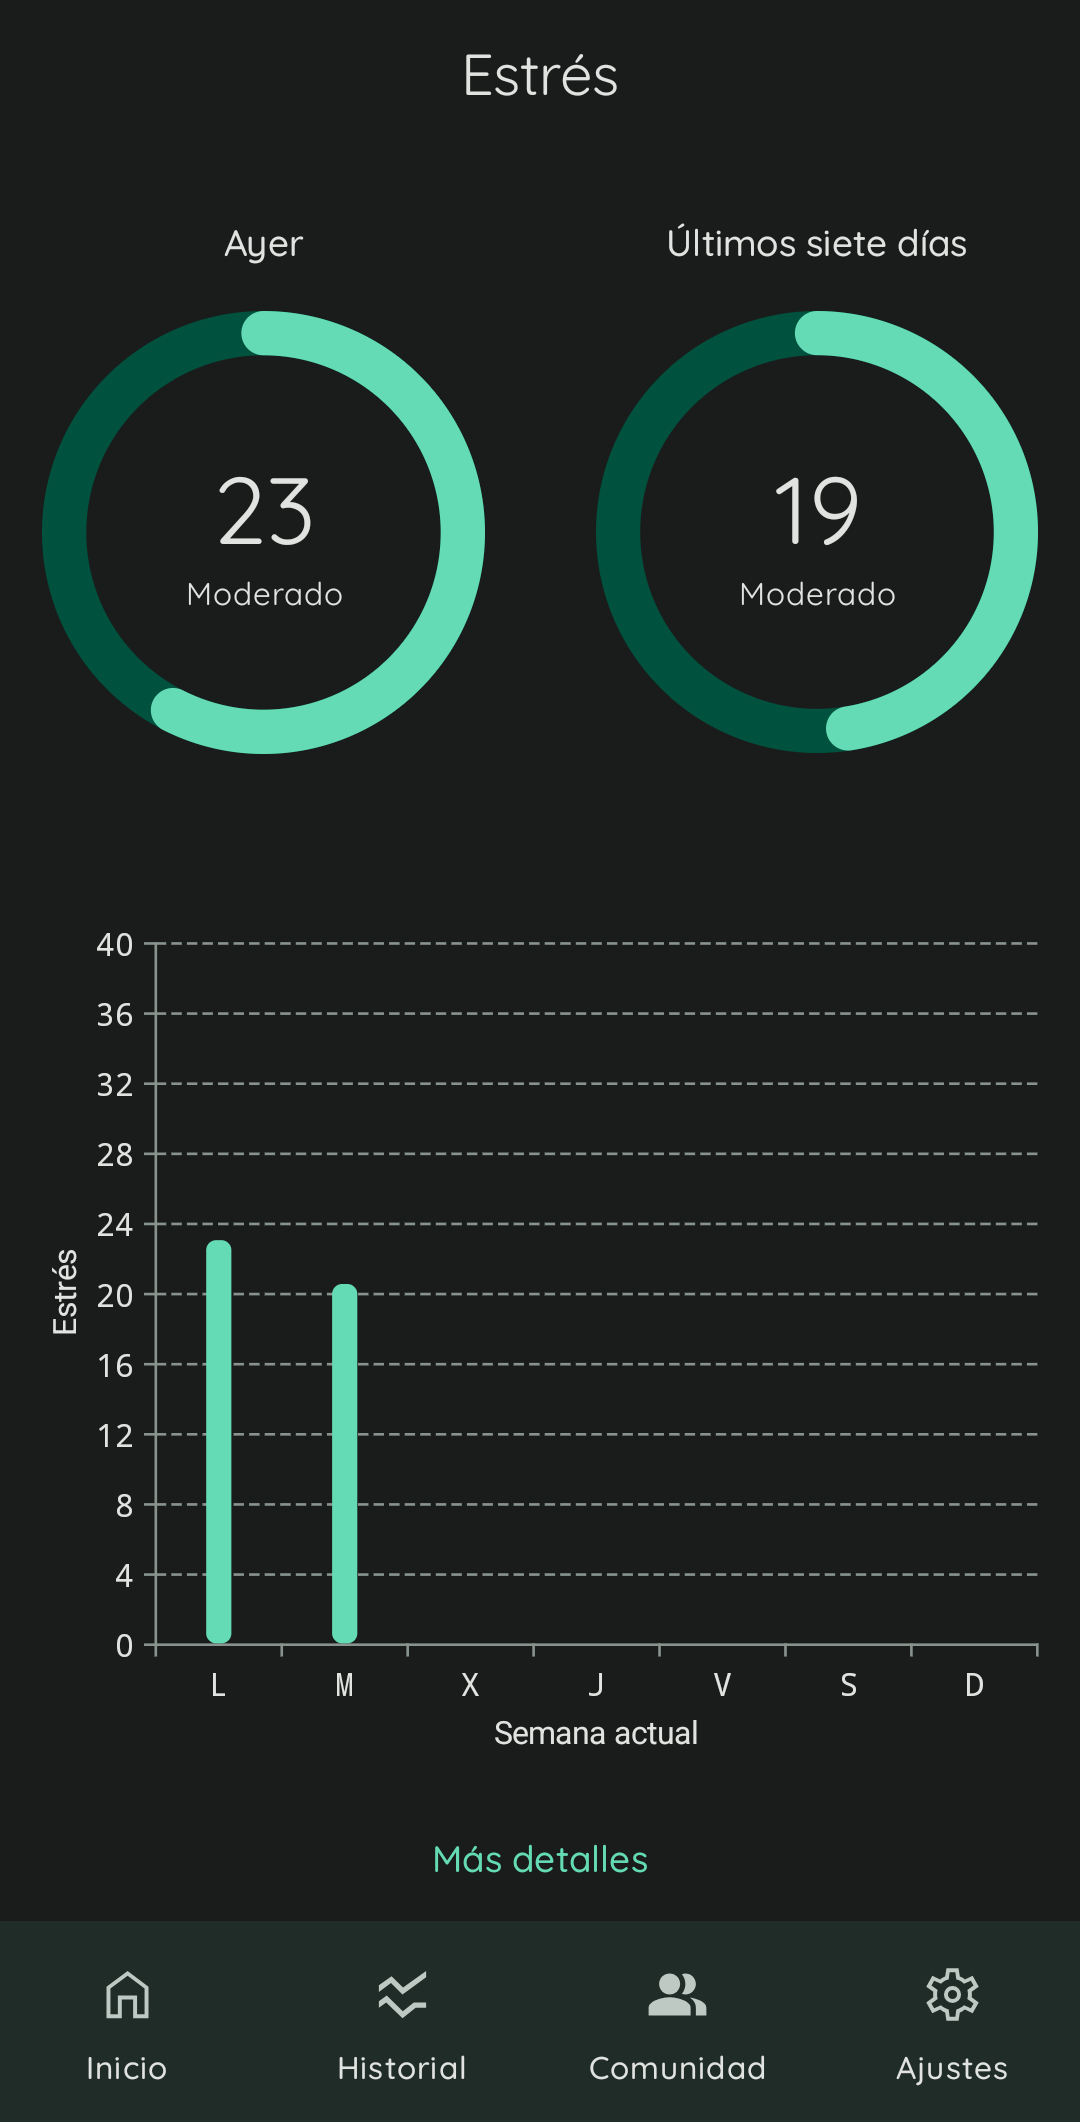
\includegraphics[width=1\textwidth]{figures/pantallas/Medida.png}
                	\end{subfigure}
                	\hspace{0.1\textwidth}
                	\begin{subfigure}[c]{0.4\textwidth}
                		\centering
                		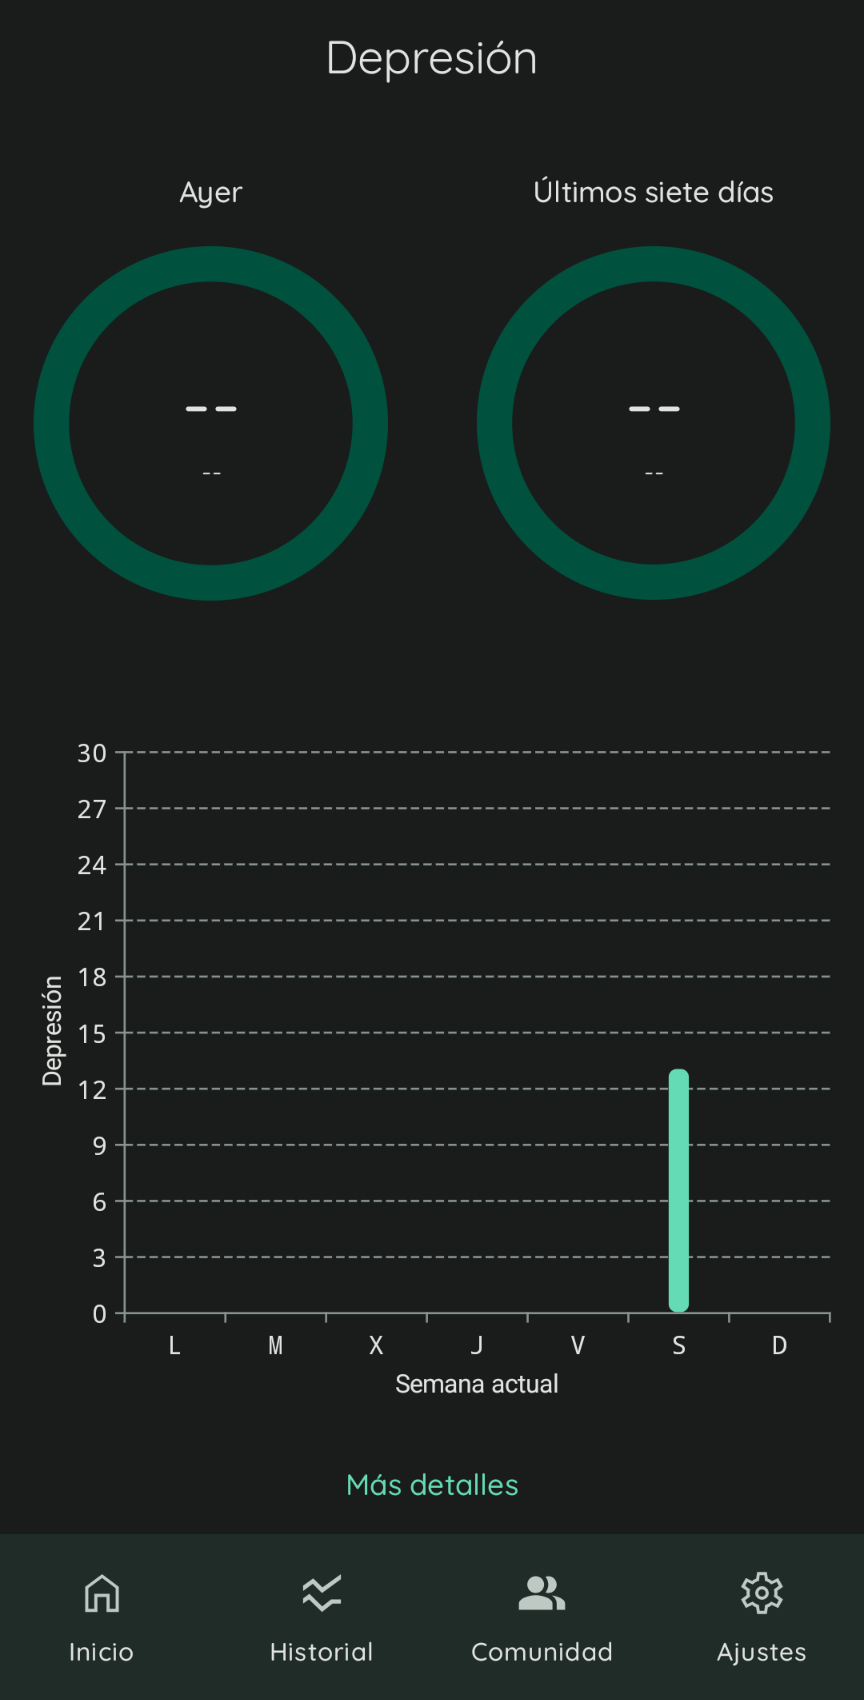
\includegraphics[width=1\linewidth]{figures/pantallas/Medida con nulos.png}
                	\end{subfigure}
                	\caption{Pantalla medida}
                	\label{figure:implementacion:pantalla:medida}
                \end{figure}

                \clearpage  % Asegura que todas las figuras y tablas pendientes se impriman antes de continuar.

            \subsubsection*{Mis datos}
                En esta pantalla básica el usuario puede visualizar sus datos de actividad física, como se puede ver en la Figura \ref{figure:implementacion:pantalla:mis_datos}.

                Cuando el usuario entra en esta ventana se muestra una lista de desplegables, uno por cada tipo de dato, mientras que al abrirse uno de estos desplegables se muestran los registros de la medida en cuestión en forma de tarjetas.
                
                \begin{figure}[htbp]
                	\centering
                	\begin{subfigure}[c]{0.4\textwidth}
                		\centering
                		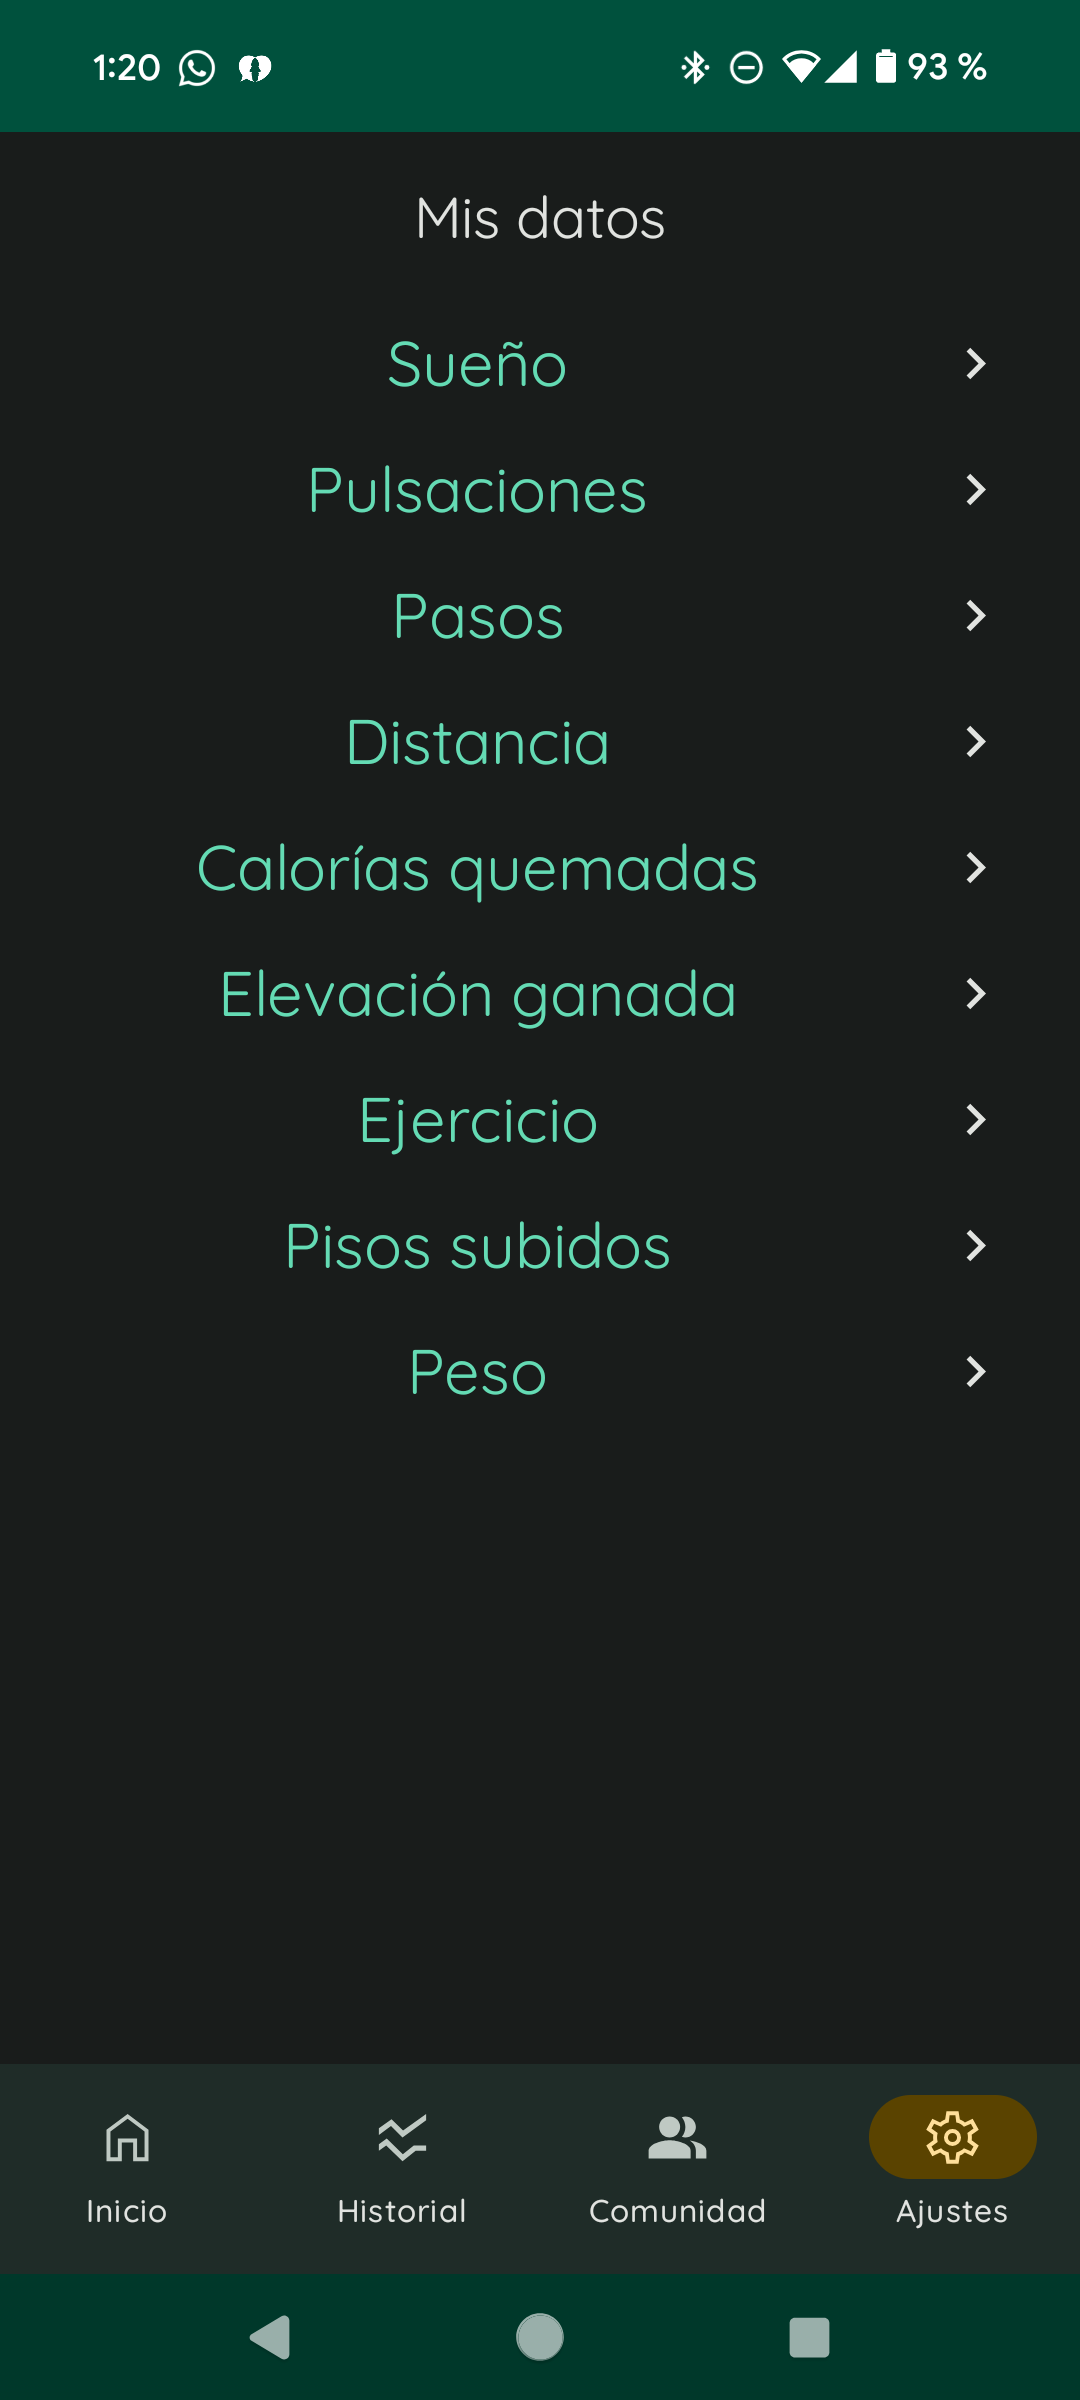
\includegraphics[width=1\textwidth]{figures/pantallas/Mis datos.png}
                	\end{subfigure}
                	\hspace{0.1\textwidth}
                	\begin{subfigure}[c]{0.4\textwidth}
                		\centering
                		\includegraphics[width=1\linewidth]{figures/pantallas/Datos sueño.png}
                	\end{subfigure}
                	\caption{Pantalla \textit{mis datos}}
                	\label{figure:implementacion:pantalla:mis_datos}
                \end{figure}	

                \clearpage  % Asegura que todas las figuras y tablas pendientes se impriman antes de continuar.
            
            \subsubsection*{Privacidad}
                Esta ventana básica, únicamente accesible desde ajustes, contiene el mismo diseño que la pantalla de consejo: el texto en cuestión y el botón de vuelta atrás. 

                La Figura \ref{figure:implementacion:pantalla:privacidad} muestra la pantalla de privacidad disponible en el usuario. Puede verse que la política de privacidad no se acabó diseñando durante la fase de implementación de este \gls{tfm}. 
                
                \begin{figure}[h]
                	\centering
                	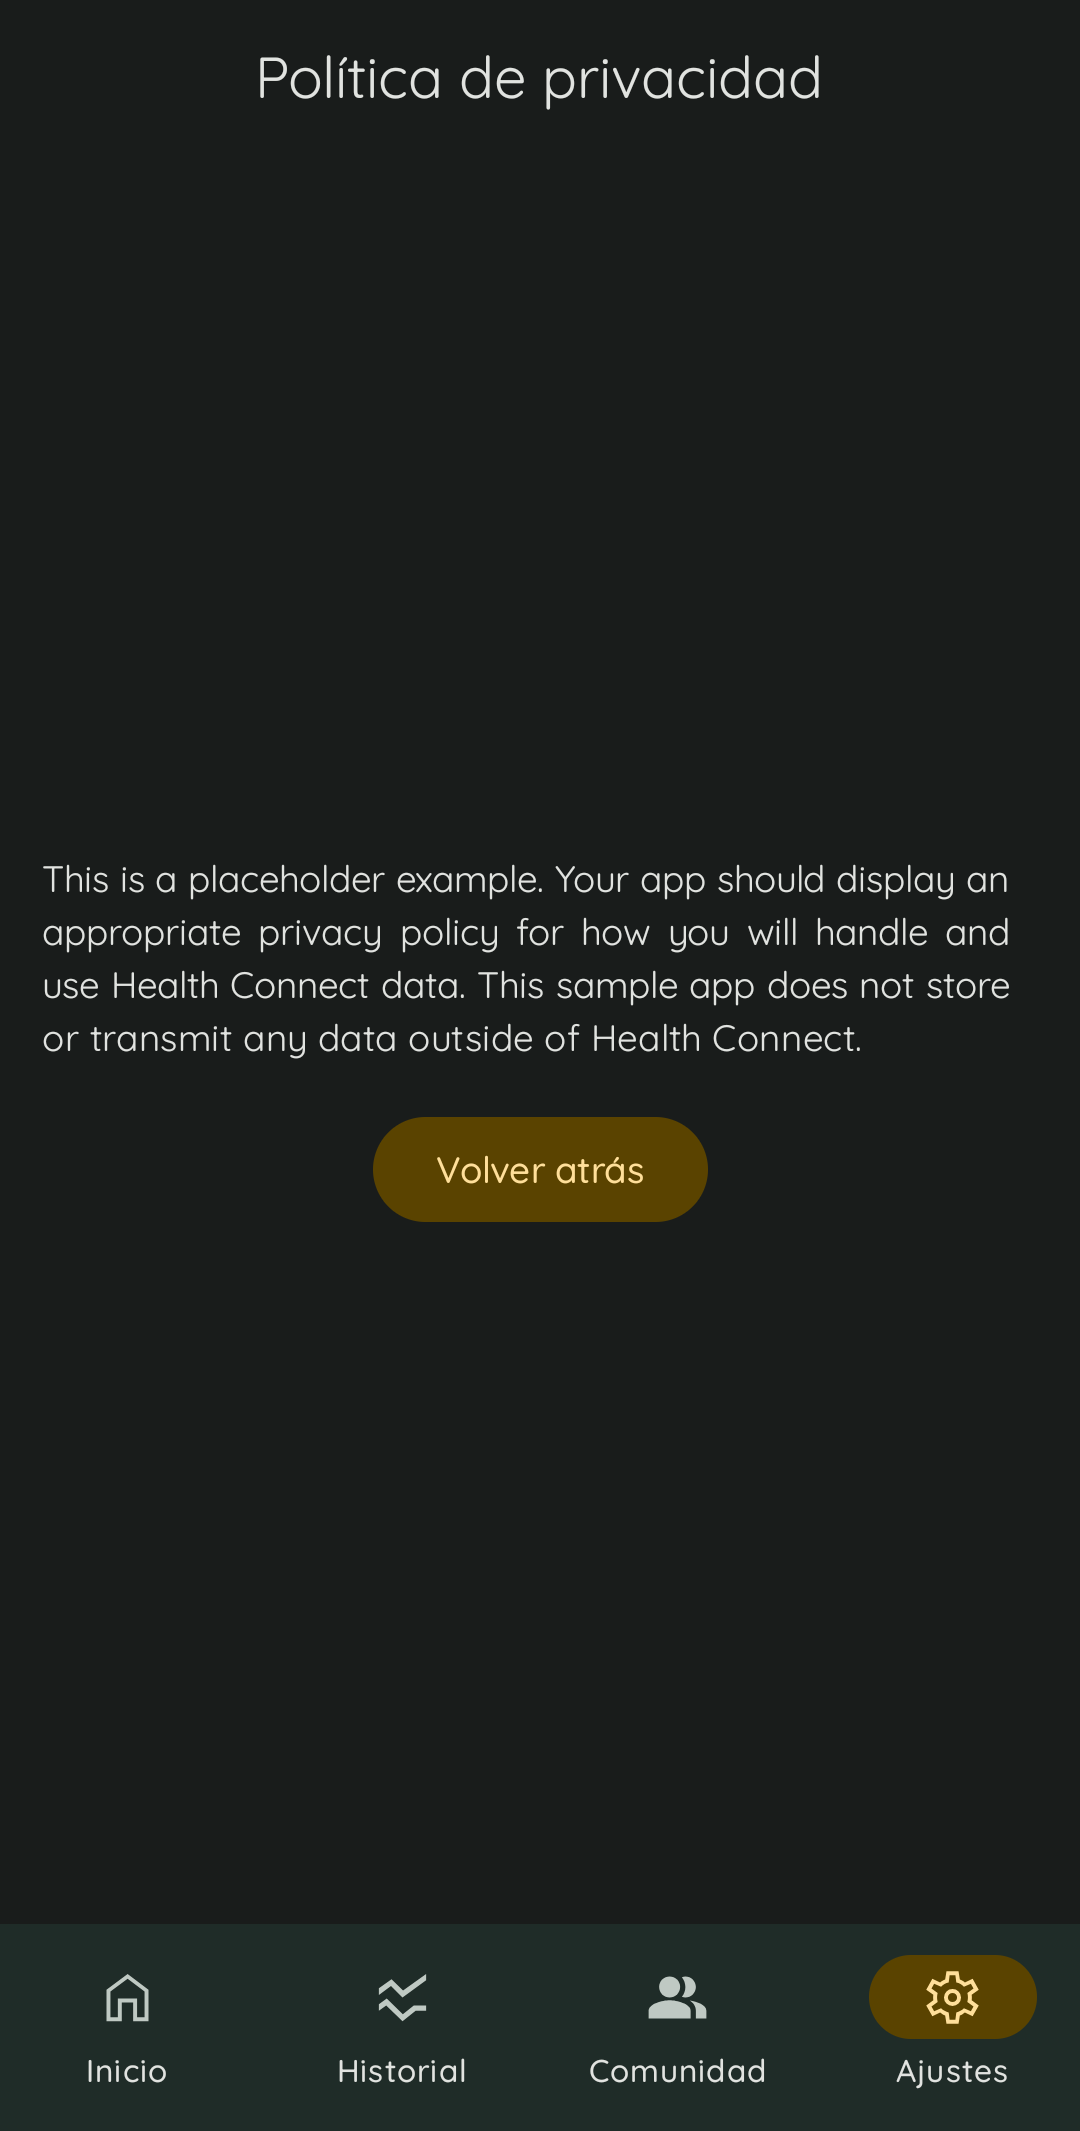
\includegraphics[width=0.4\textwidth]{figures/pantallas/Privacidad.png}
                	\caption{Pantalla privacidad}
                	\label{figure:implementacion:pantalla:privacidad}
                \end{figure}

                \clearpage  % Asegura que todas las figuras y tablas pendientes se impriman antes de continuar.
            
                
            \subsubsection*{Acerca de}
                Se trata de una pantalla idéntica al caso anterior, cambiando la política de privacidad por los datos de la aplicación. La Figura \ref{figure:implementacion:pantalla:acerca_de} muestra esta ventana.
                
                \begin{figure}[h]
                	\centering
                	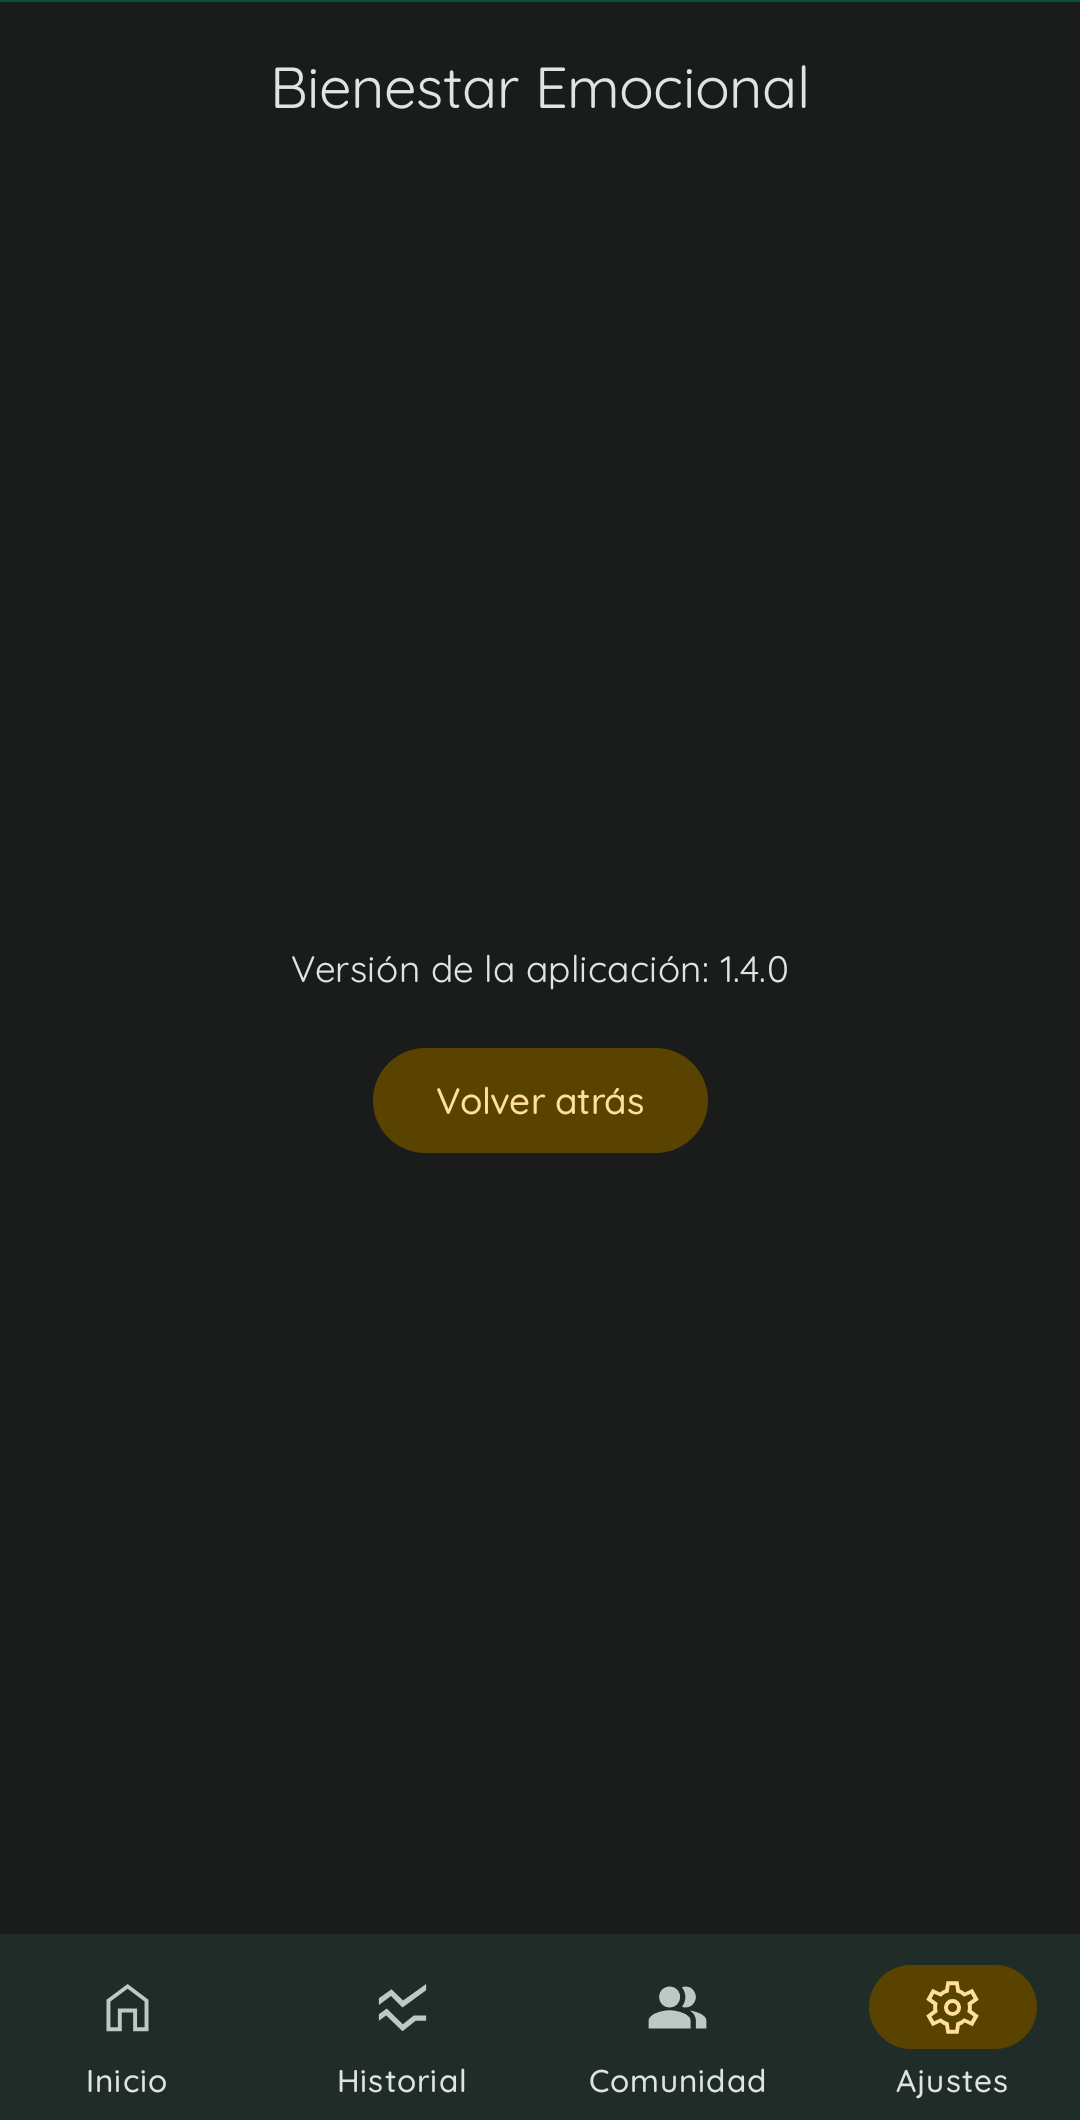
\includegraphics[width=0.4\textwidth]{figures/pantallas/Acerca de.png}
                	\caption{Pantalla \textit{acerca de}}
                	\label{figure:implementacion:pantalla:acerca_de}
                \end{figure}

                \clearpage  % Asegura que todas las figuras y tablas pendientes se impriman antes de continuar.
            \subsubsection*{Créditos}
                Esta ventana básica contiene la lista de las personas que han trabajado en el desarrollo de la aplicación junto con su papel en la misma. También se dan créditos a las personas que han creado algunos de los elementos gráficos utilizados por la aplicación.

                La Figura \ref{figure:implementacion:pantalla:creditos} representa cómo se ven los créditos en la aplicación\footnote{La aplicación muestra una errata: María no es coautora de este proyecto, sino autora de su propio proyecto basado en este \gls{tfm}.}.
                
                \begin{figure}[h]
                	\centering
                	\includegraphics[width=0.4\textwidth]{figures/pantallas/Créditos.png}
                	\caption{Pantalla créditos}
                	\label{figure:implementacion:pantalla:creditos}
                \end{figure}

                \clearpage  % Asegura que todas las figuras y tablas pendientes se impriman antes de continuar.
            \subsubsection*{Cuestionarios incompletos}
                Esta pantalla básica y condicional solo aparece cuando el usuario tiene cuestionarios incompletos, los cuales son agrupados por rondas. Cada ronda incompleta es presentada en forma de tarjeta, contiendo información de qué cuestionarios faltan y un botón para retomarlos, como se puede ver en la Figura \ref{figure:implementacion:pantalla:cuestionarios_incompletos}.
                
                \begin{figure}[h]
                	\centering
                	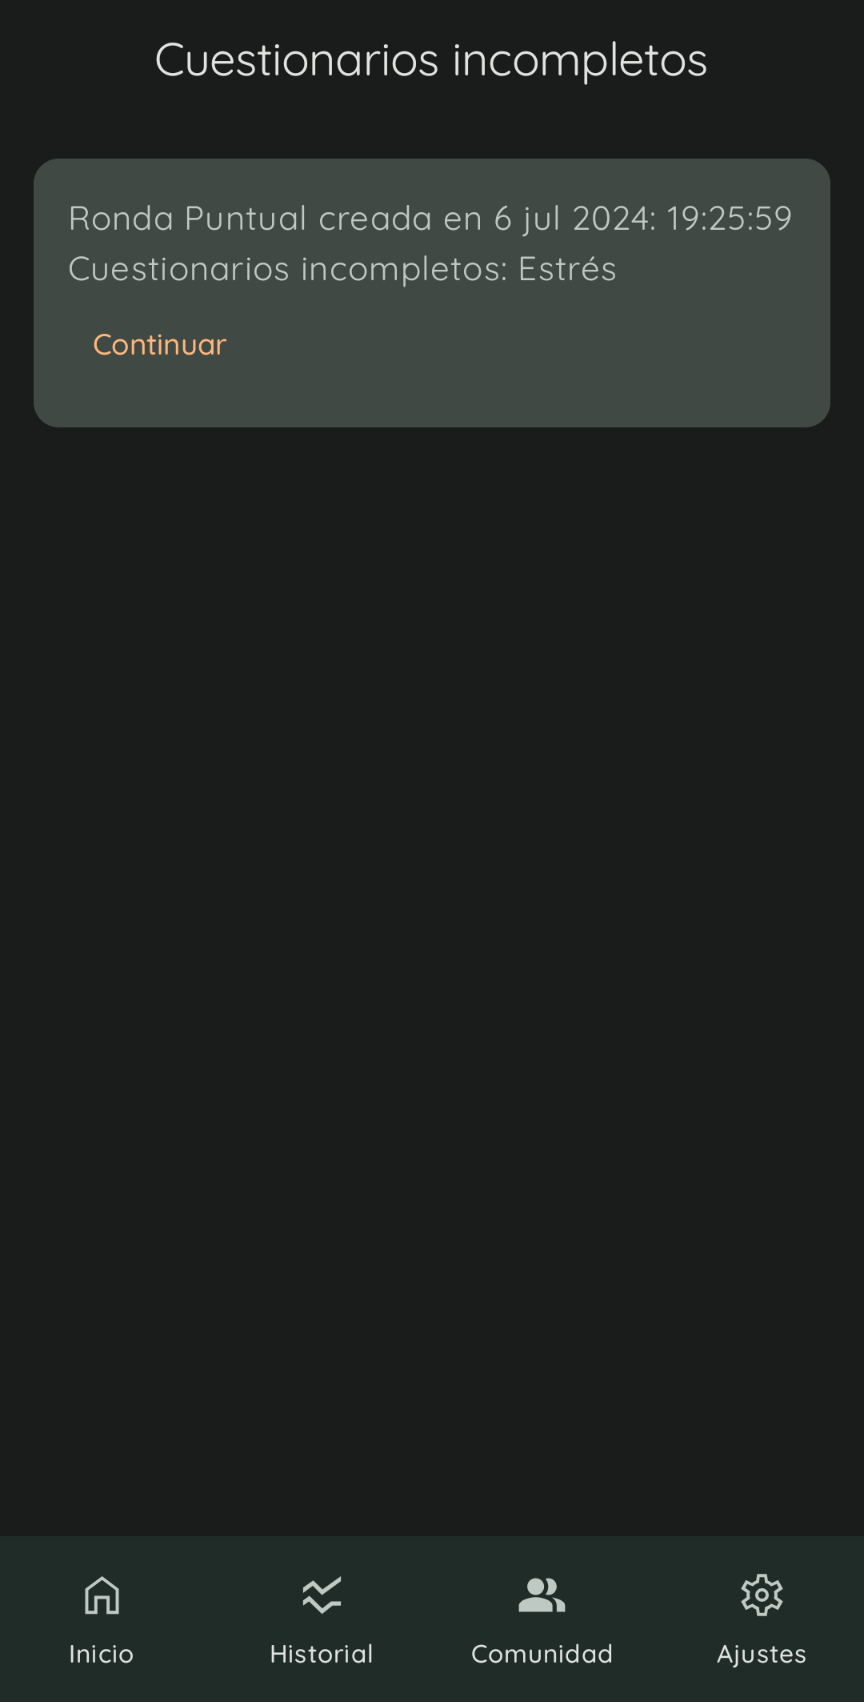
\includegraphics[width=0.4\textwidth]{figures/pantallas/Cuestionarios pendientes.png}
                	\caption{Pantalla \textit{cuestionarios incompletos}}
                	\label{figure:implementacion:pantalla:cuestionarios_incompletos}
                \end{figure}

                \clearpage  % Asegura que todas las figuras y tablas pendientes se impriman antes de continuar.
            \subsubsection*{Estrés, depresión y soledad diario}
                Debido a que las tres pantallas sólo varían en los textos presentados, se han agrupado bajo esta sección. La Figura \ref{figure:implementacion:pantalla:estres_depresion_soledad_diarios} refleja la representación de estos cuestionarios.

                \begin{figure}[htbp]
                	\centering
                	\begin{subfigure}[c]{0.29\textwidth}
                		\centering
                		\includegraphics[width=1\textwidth]{figures/pantallas/Estrés diario.png}
                	\end{subfigure}
                	\hspace{0.05\textwidth}
                	\begin{subfigure}[c]{0.29\textwidth}
                		\centering
                		\includegraphics[width=1\linewidth]{figures/pantallas/Depresión diario.png}
                	\end{subfigure}
                    \hspace{0.05\textwidth}
                	\begin{subfigure}[c]{0.29\textwidth}
                		\centering
                		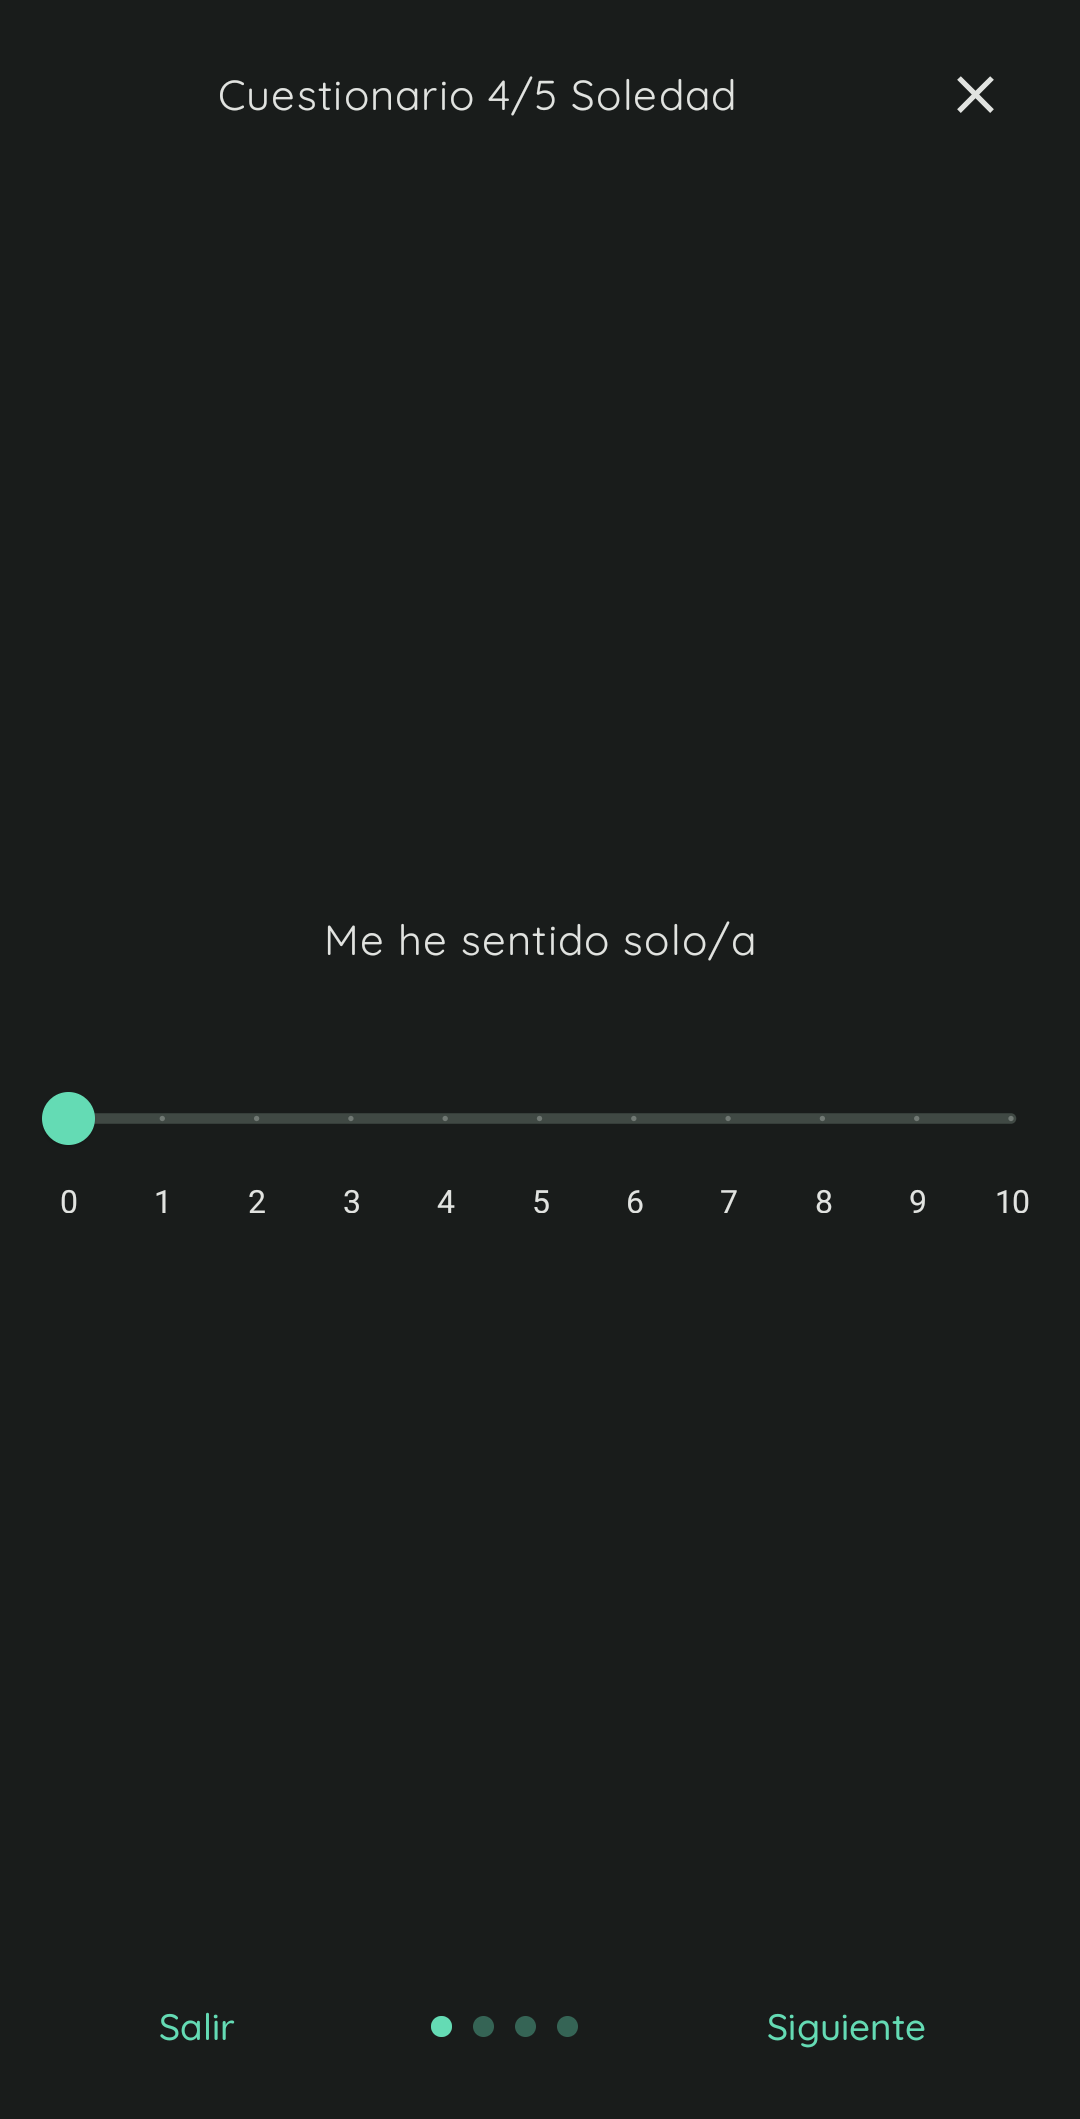
\includegraphics[width=1\linewidth]{figures/pantallas/Soledad diario.png}
                	\end{subfigure}
                	\caption{Pantallas estrés, depresión y soledad diarios}
                	\label{figure:implementacion:pantalla:estres_depresion_soledad_diarios}
                \end{figure}

                En este caso se puede ver que las preguntas están dispuestas en forma de carrousel con botones para salir o pasar a la siguiente, siendo un patrón que se repetirá para todos los cuestionarios. Además se presenta una barra en la parte superior que indica el número de cuestionario dentro de la ronda, cuál es y un botón para omitirlo.

                En este caso, como la respuesta a la pregunta es numérica, el usuario dispone de una escala gráfica que puede pulsar para responder.

                Por otra parte la Figura \ref{figure:implementacion:pantalla:dialogos_cuestionarios} muestra los diferentes avisos que se pueden mostrar para todos los cuestionarios de la aplicación, en particular el de \textit{preguntas restantes} y el de \textit{omitir cuestionario}.
                
                \begin{figure}[htbp]
                	\centering
                	\begin{subfigure}[c]{0.29\textwidth}
                		\centering
                		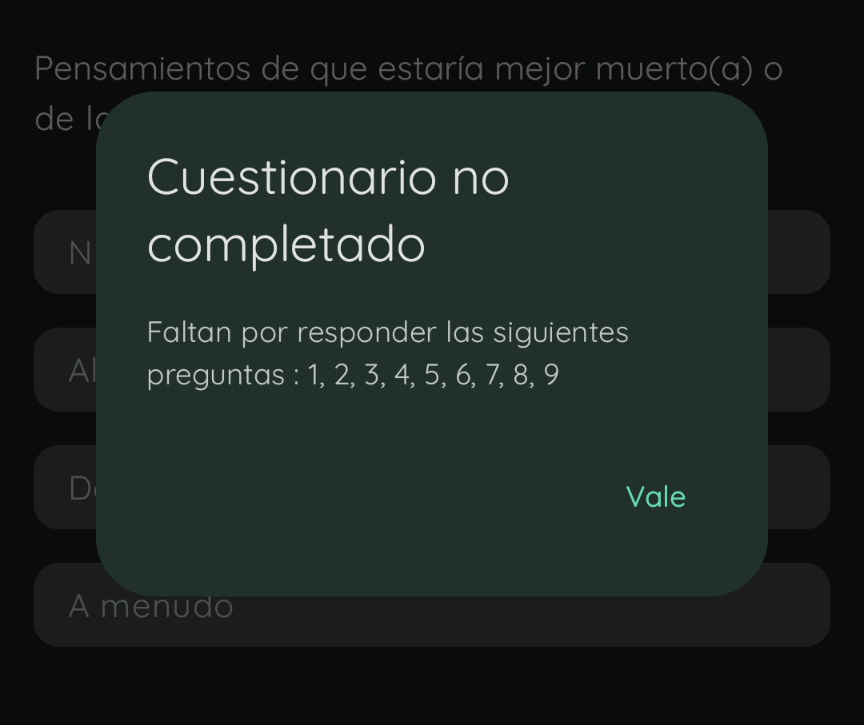
\includegraphics[width=1\textwidth]{figures/pantallas/Preguntas restantes.png}
                	\end{subfigure}
                	\hspace{0.05\textwidth}
                	\begin{subfigure}[c]{0.29\textwidth}
                		\centering
                		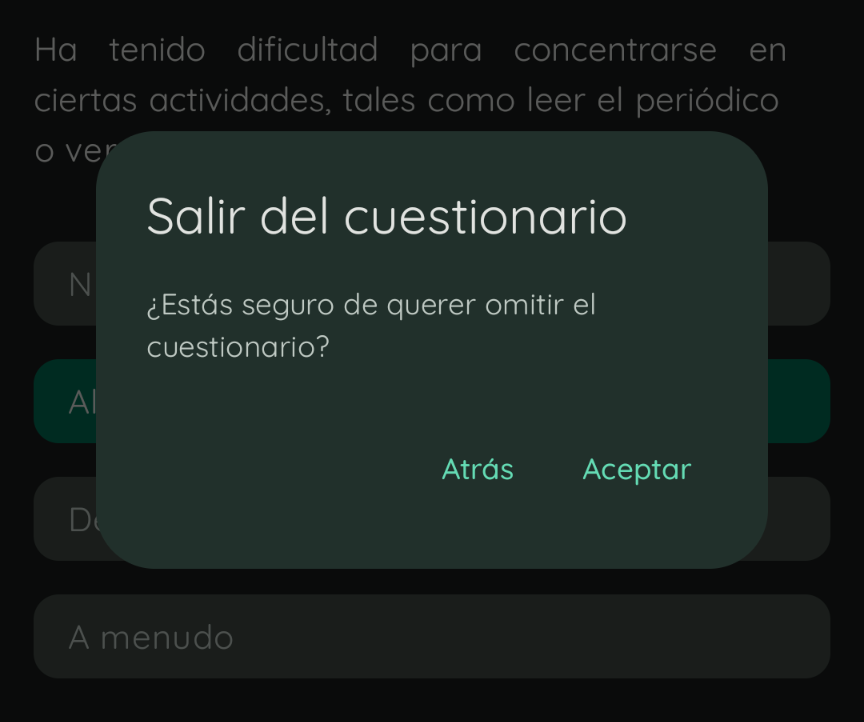
\includegraphics[width=1\linewidth]{figures/pantallas/Salir del cuestionario.png}
                	\end{subfigure}
                	\caption{Diálogos de los cuestionarios de la aplicación}
                	\label{figure:implementacion:pantalla:dialogos_cuestionarios}
                \end{figure}

                Por último la Figura \ref{figure:implementacion:pantalla:diarios_resumen} representa los elementos resumen que se muestran al finalizar los cuestionarios de estrés, depresión y soledad diarios.

                \begin{figure}[h]
                	\centering
                	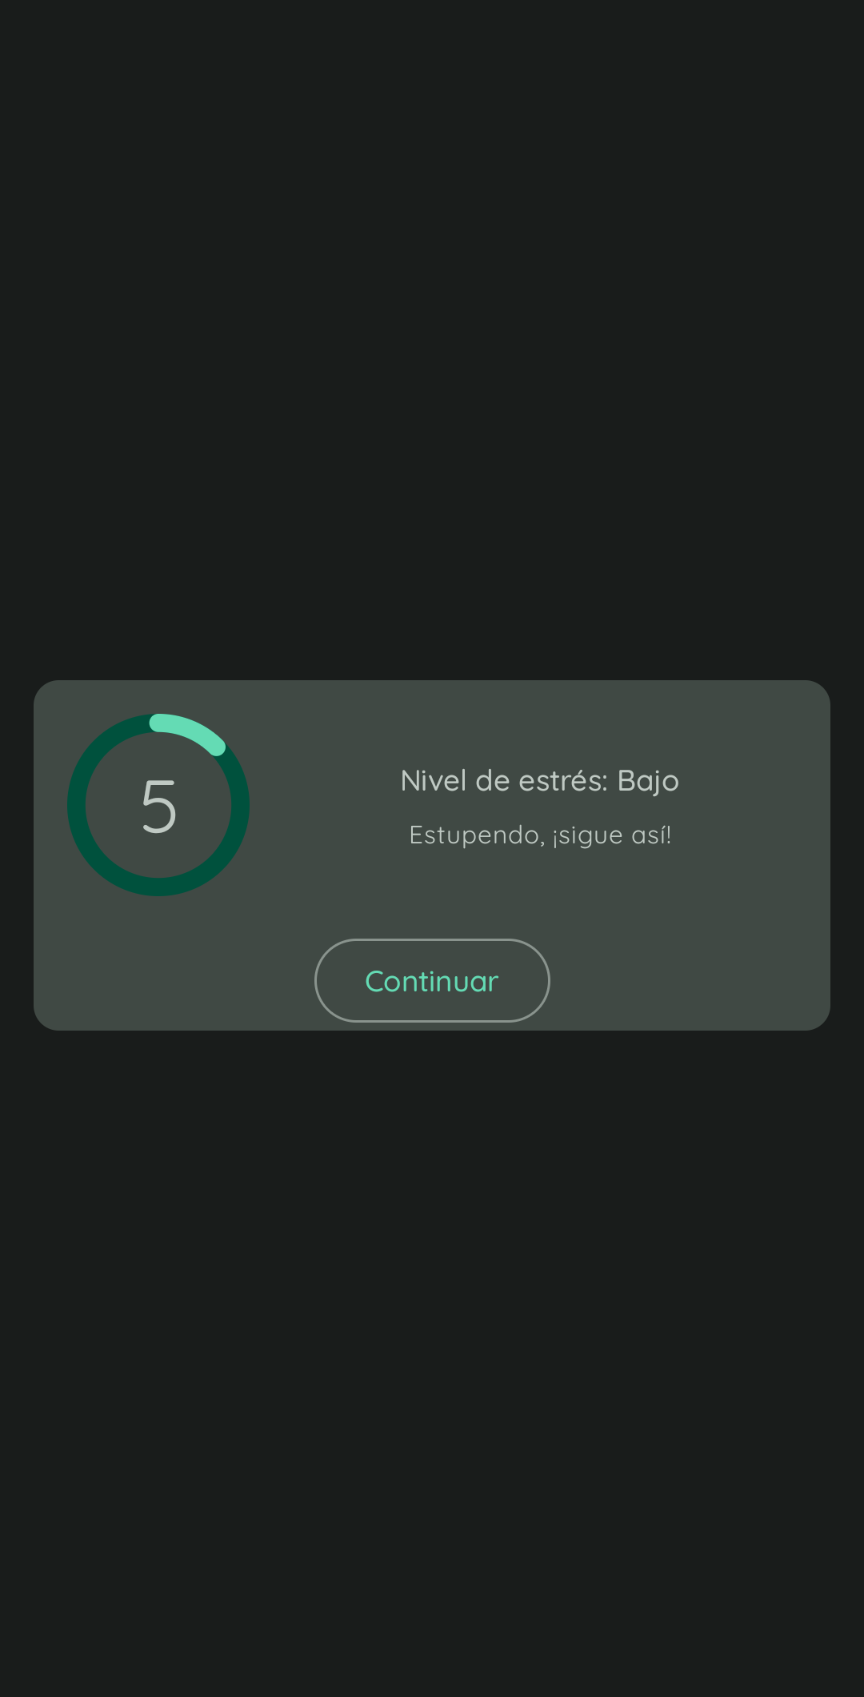
\includegraphics[width=0.4\textwidth]{figures/pantallas/Resumen cuestionario.png}
                	\caption{Resumen de los cuestionarios estrés, depresión y soledad diarios}
                	\label{figure:implementacion:pantalla:diarios_resumen}
                \end{figure}

                \clearpage  % Asegura que todas las figuras y tablas pendientes se impriman antes de continuar.
            \subsubsection*{Suicidio diario}
                Este cuestionario presenta a diferencia de los tres anteriores preguntas de selección, con la particularidad de que si el usuario marca una respuesta como \textit{no} el cuestionario finaliza, ya que las preguntas ahondan sucesivamente en mayor riesgo de depresión.
                
                La Figura \ref{figure:implementacion:pantalla:suicidio_diario} muestra tanto la primera pregunta del cuestionario como el resumen que se presenta a la finalización del mismo ejemplificado en riesgo alto.

                \begin{figure}[htbp]
                	\centering
                	\begin{subfigure}[c]{0.4\textwidth}
                		\centering
                		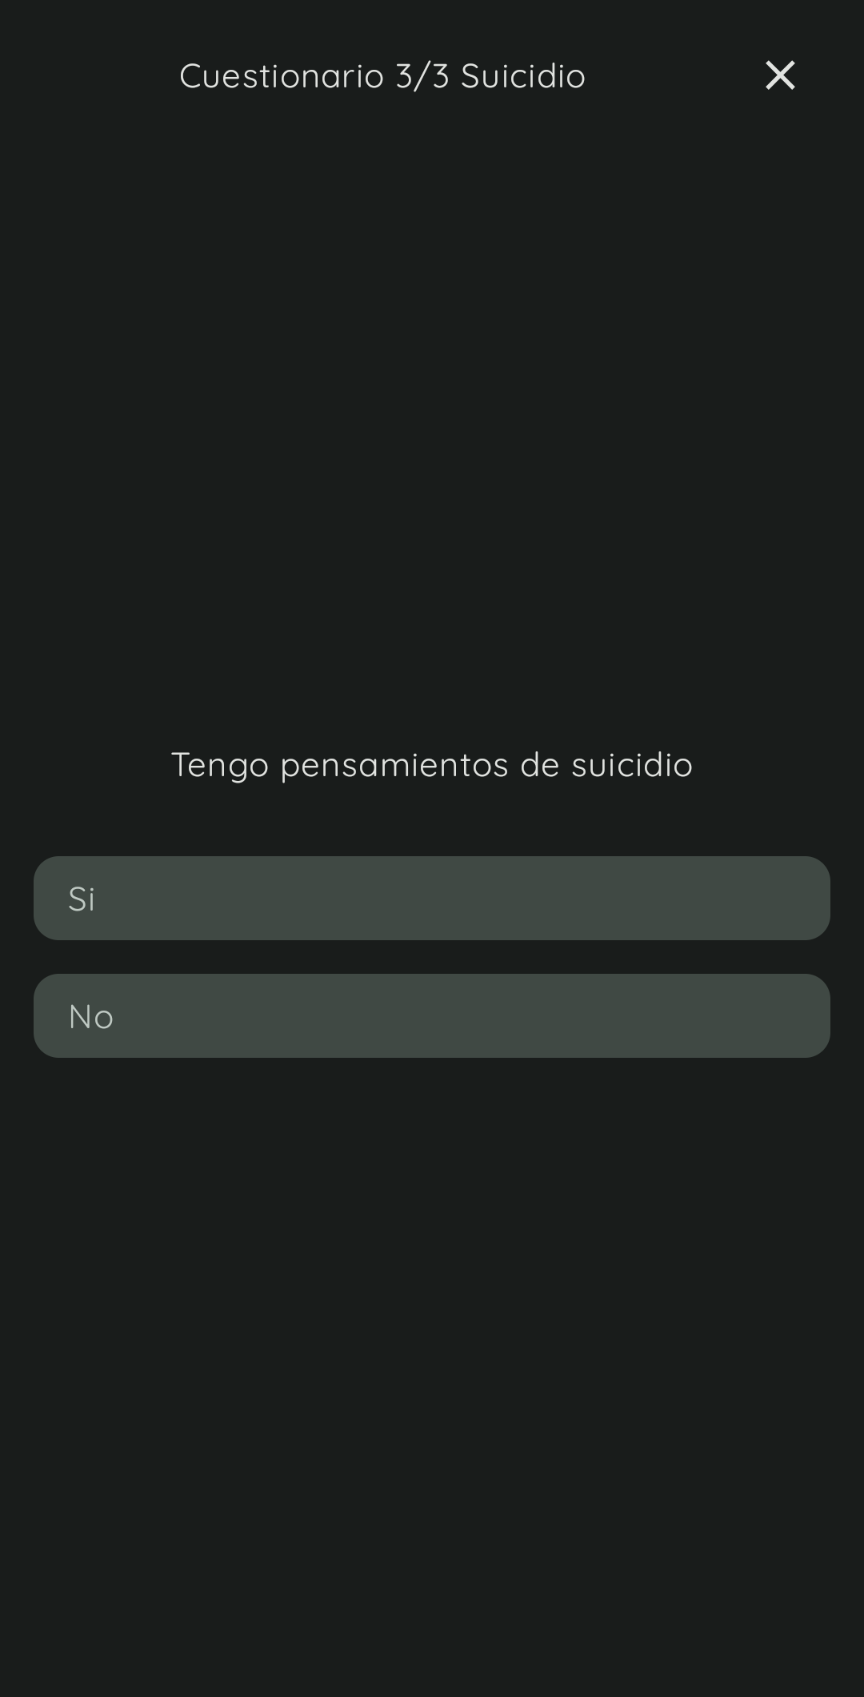
\includegraphics[width=1\textwidth]{figures/pantallas/Suicidio diario.png}
                	\end{subfigure}
                	\hspace{0.1\textwidth}
                	\begin{subfigure}[c]{0.4\textwidth}
                		\centering
                		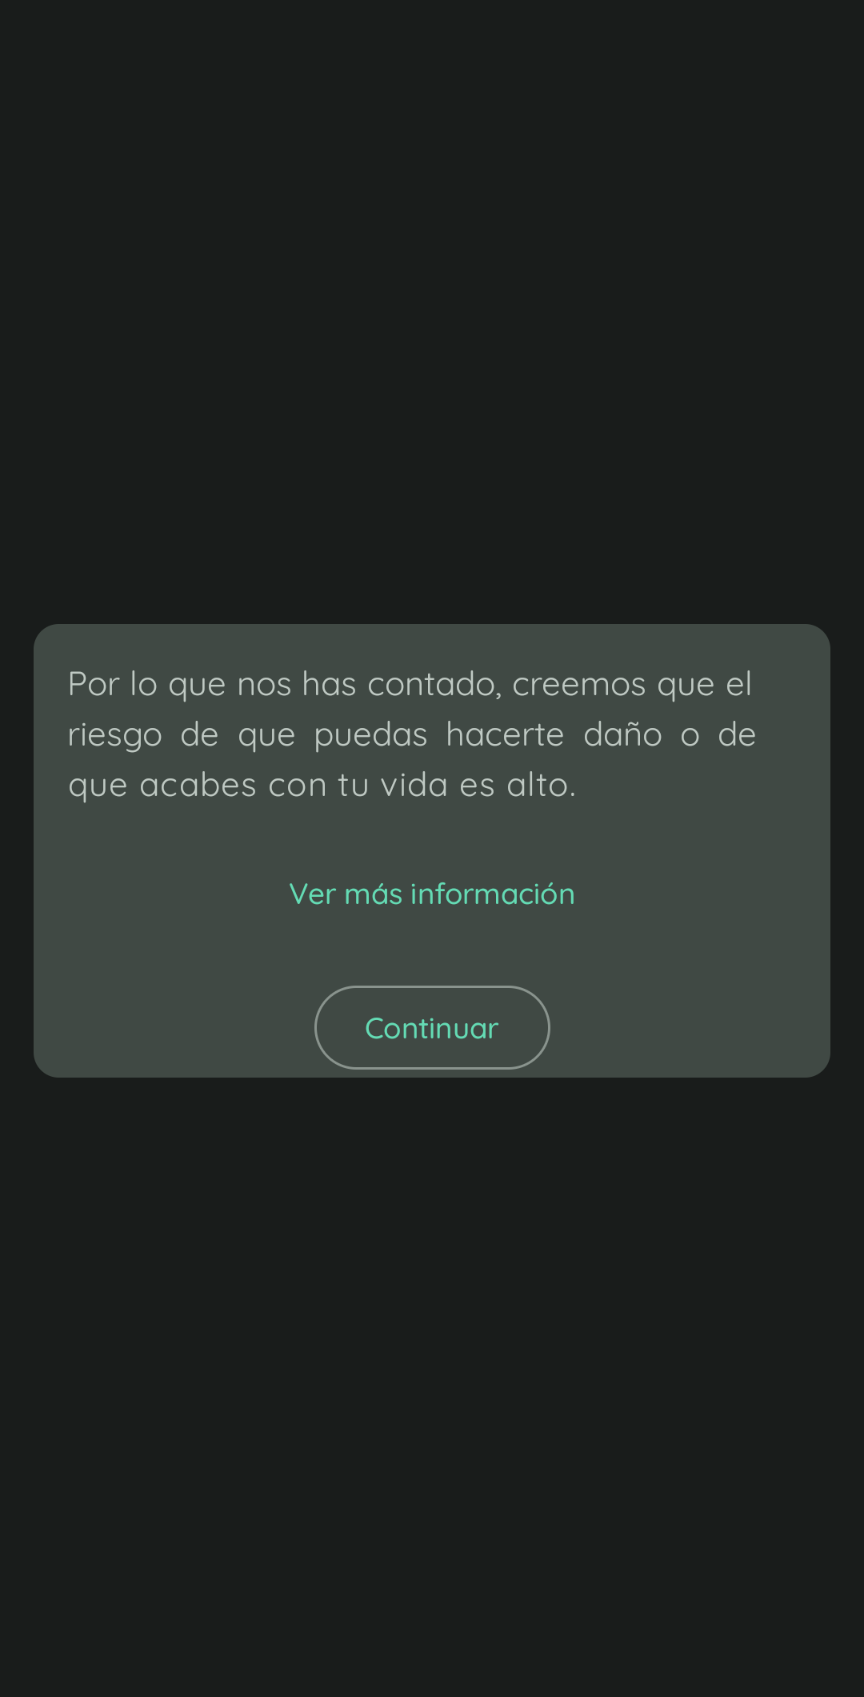
\includegraphics[width=1\linewidth]{figures/pantallas/Resumen suicidio.png}
                	\end{subfigure}
                	\caption{Pantalla y resumen del cuestionario \textit{suicidio diario}}
                	\label{figure:implementacion:pantalla:suicidio_diario}
                \end{figure}
                

                \clearpage  % Asegura que todas las figuras y tablas pendientes se impriman antes de continuar.
            \subsubsection*{Contraste diario}
                Este cuestionario presenta preguntas de selección, con la particularidad de no presentar resumen a la finalización del mismo al no disponer de puntuación o nivel de medida. La Figura \ref{figure:implementacion:pantalla:contraste_diario} presenta la primera pregunta del cuestionario contraste. 
                
                \begin{figure}[h]
                	\centering
                	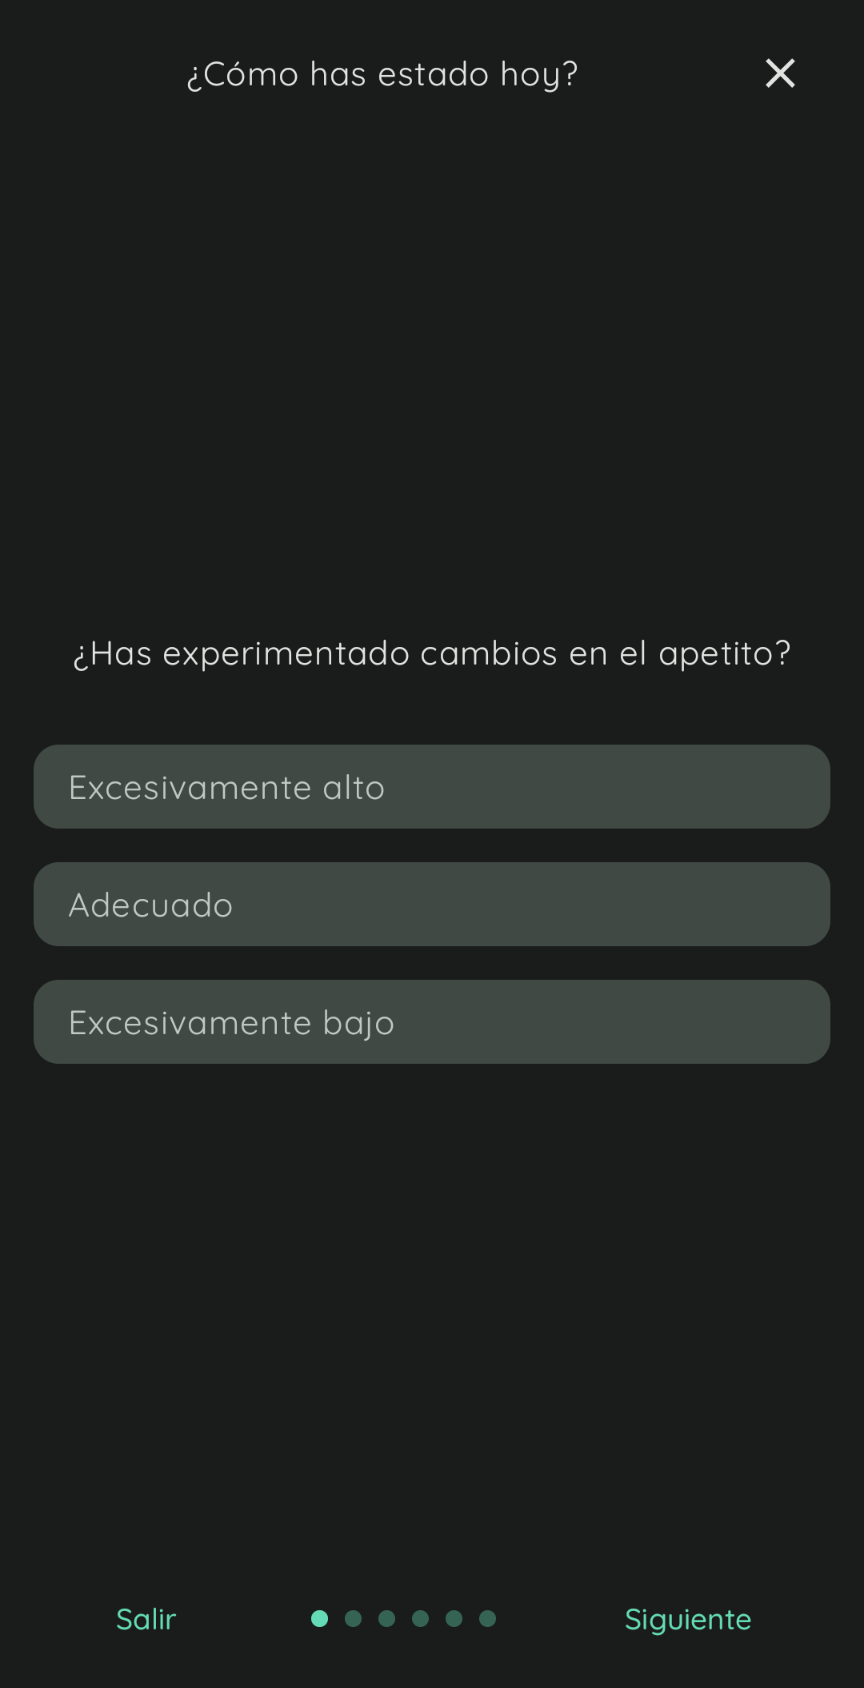
\includegraphics[width=0.4\textwidth]{figures/pantallas/Contraste diario.png}
                	\caption{Pantalla \textit{contraste diario}}
                	\label{figure:implementacion:pantalla:contraste_diario}
                \end{figure}

                \clearpage  % Asegura que todas las figuras y tablas pendientes se impriman antes de continuar.
            \subsubsection*{Estrés, depresión y soledad puntual}
                Por último, como sus homólogos diarios, estos tres cuestionarios solo varían en los textos y las opciones disponibles para responder, por lo que han sido agrupados nuevamente. La única diferencia con respecto a sus variantes diarias reside en el uso de respuestas cualitativas.
                
                La Figura \ref{figure:implementacion:pantalla:puntuales} refleja la representación de estos cuestionarios.
                
                \begin{figure}[htbp]
                	\centering
                	\begin{subfigure}[c]{0.29\textwidth}
                		\centering
                		\includegraphics[width=1\textwidth]{figures/pantallas/Estrés puntual.png}
                	\end{subfigure}
                	\hspace{0.05\textwidth}
                	\begin{subfigure}[c]{0.29\textwidth}
                		\centering
                		\includegraphics[width=1\linewidth]{figures/pantallas/Depresión puntual.png}
                	\end{subfigure}
                    \hspace{0.05\textwidth}
                	\begin{subfigure}[c]{0.29\textwidth}
                		\centering
                		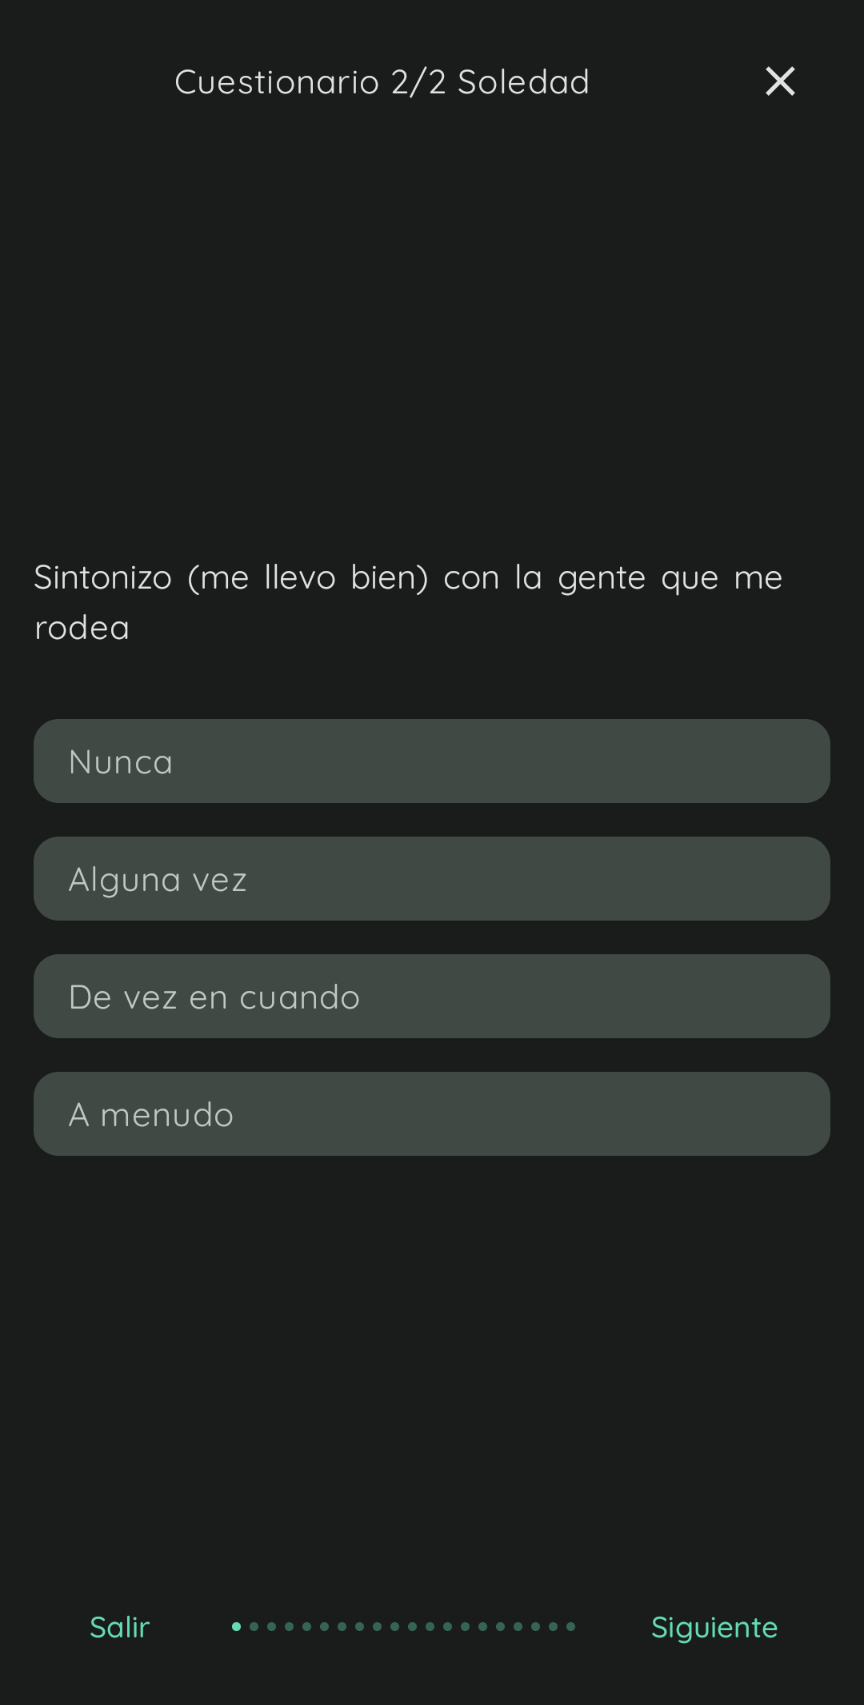
\includegraphics[width=1\linewidth]{figures/pantallas/Soledad puntual.png}
                	\end{subfigure}
                	\caption{Pantallas de los cuestionarios puntuales}
                	\label{figure:implementacion:pantalla:puntuales}
                \end{figure}
                
                \clearpage  % Asegura que todas las figuras y tablas pendientes se impriman antes de continuar.
        
        \subsection{Librerías utilizadas}
            \label{section:implementacion:librerias_app}
            Si bien en la Sección \ref{section:contexto} se detallaron las tecnologías más destacadas utilizadas para el desarrollo de la aplicación, las siguientes librerías también fueron utilizadas:
            \begin{itemize}
                \item \href{https://developer.android.com/training/dependency-injection/hilt-android}{\textit{Dagger Hilt}} para la inyección de dependencias.
                \item \href{https://github.com/google/accompanist}{\textit{Accompanist}} como extensión de \textit{Jetpack Compose} para la implementación del carrousel.
                \item \href{https://developer.android.com/topic/libraries/architecture/datastore}{\textit{Datastore}} para el guardado en disco de los ajustes de la aplicación, los cuales no fueron incluidos en el diagrama Entidad Relación.
                \item \href{https://github.com/raamcosta/compose-destinations}{\textit{Compose Destinations}} para mejorar la navegación entre pantallas, concretamente para permitir el paso de objetos entre ellas.
                \item \href{https://github.com/alorma/Compose-Settings}{\textit{Compose Settings}} para la implementación de componentes gráficos no incluidos en \textit{Material Design 3}, como los \textit{switches} del menú de ajustes o los diálogos de selección.
                \item \href{https://github.com/YarikSOffice/lingver}{\textit{Lingver}} para el cambio de idioma, ya que por defecto Android toma el lenguaje o \textit{locale} del sistema y no permite cambiarlo.
                \item \href{https://github.com/sqlcipher/android-database-sqlcipher}{\textit{Sqlcipher}} para el cifrado \gls{aes} de la base de datos Room.
                \item \href{https://github.com/square/retrofit}{\textit{Retrofit}} como cliente \gls{http} para la realización de llamadas a la \gls{api} del servidor.
            \end{itemize}
            \clearpage  % Asegura que todas las figuras y tablas pendientes se impriman antes de continuar.
    \section{Servidor}
        
        A diferencia del caso anterior, la implementación de este componente resulta trivial a partir de los diagramas realizados en la fase de diseño. La codificación se ha realizado mediante el uso de \textit{Python} como lenguaje principal, \textit{Flask} como \gls{microframework} para la realización de la \gls{api} y \textit{pymongo} para interactuar con MongoDB. 

        Los aspectos a destacar de esta implementación son:
        \begin{itemize}
            \item Se dispone un \textit{endpoint} para el acceso a cada colección.
            \item El módulo \textit{validator} realiza las comprobaciones del formato del \gls{payload} que contiene los datos a insertar. En caso de que la verificación sea exitosa la \gls{api} responderá con un código de éxito (independientemente de si se inserten datos o no), devolviendo en caso contrario un código de error.
            \item Sólo se insertan datos si el formato del \gls{payload} es válido y contiene datos para añadir a la base de datos.
            \item Se añadieron trazas o \textit{logs} para cada acción relevante.
        \end{itemize}

        En cuanto al despliegue del componente, se realizó en un servidor de la \gls{etsisi} que dispone de sistema operativo Ubuntu, el cual aloja también la base de datos. Para la visualización de los datos fue instalado el entorno gráfico \textit{robo3t}, mientras el acceso al propio servidor fue realizado mediante el uso de clientes \gls{ssh} con la extensión \textit{x11} para el soporte del sistema de ventanas. 